 % -*- mode: LaTeX -*-
 % ... preamble ...
\documentclass[times,12pt,titlepage]{mstogs}
\doublespacing
\usepackage[authoryear,sort]{natbib} % ... numbers or authoryear ...
\setlength{\bibhang}{0.5in}
\usepackage{threeparttable}
\usepackage[final]{graphicx}
\usepackage{psfrag}
\usepackage[noprefix]{nomencl}

\usepackage{booktabs}
\usepackage{caption}
\usepackage{subcaption}
\usepackage{algorithm}
\usepackage{algpseudocode}
\usepackage[utf8]{inputenc}

\makenomenclature
 % ... nomenclature groupings ...
\renewcommand{\nomgroup}[1]{
   \ifthenelse{\equal{#1}{A}}{\medskip \item \textbf{Roman}}{}%
   \ifthenelse{\equal{#1}{G}}{\medskip \item \textbf{Greek}}{}%
   \ifthenelse{\equal{#1}{S}}{\medskip \item \textbf{Subscripts}}{}%
}
 % ... nomenclature preamble ...
\renewcommand{\nompreamble}{%
\hspace*{-0.50in}\makebox[1.0in][l]{Symbol} Description}
\renewcommand{\nomlabelwidth}{1.0in}

 % ... end preamble ...

\begin{document}

 % ... specify: ms or phd ...

\begin{ThesisTitlePage}{ms}

 % ... title page info ...

\author{\MakeUppercase{Samuel Nathan Richter}}

\thesistitle{\MakeUppercase{Evolved Parameterized Selection of Evolutionary Algorithms}}

\department{Computer Science}

 % ... thesis committee ...

\ThesisAdvisor{Daniel Tauritz, Advisor}

\ThesisCommittee{%
Patrick Taylor\\ %
Samuel Mulder}

 % ... Graduation date - NOT your submission date ...
\graddate{2018}

\end{ThesisTitlePage}
 % ... copyright page - true|false ...

\copyrightyear{2018}
\ThesisCopyrightPage{true}

 % ... front matter - thesis abstract ...

\begin{ThesisAbstract}
Selection functions enable Evolutionary Algorithms (EAs) to apply selection pressure to a population of individuals, by regulating the probability that an individual's genes survive, typically based on fitness. Various conventional fitness based selection functions exist, each providing a unique method of selecting individuals based on their fitness, fitness ranking within the population, and/or various other factors. However, the full space of selection algorithms is only limited by max algorithm size, and each possible selection algorithm is optimal for some EA configuration applied to a particular problem class. Therefore, improved performance may be expected by tuning an EA's selection algorithm to the problem at hand, rather than employing a conventional selection function. This thesis details an investigation of the extent to which performance can be improved by tuning selection algorithms, employing a Hyper-heuristic to explore the space of algorithms which determine the methods used to select individuals from the population. We show, with both a conventional Evolutionary Algorithm and a Covariance Matrix Adaptation Evolutionary Strategy, the increase in performance obtained with a tuned selection algorithm, versus conventional selection functions, on instances from several benchmark problem classes, including separate testing instances to show generalization of the improved performance. This thesis consists of work that was presented at the Genetic and Evolutionary Computation Conference (GECCO) in 2018, as well as work that will be submitted to GECCO in 2019. 
\end{ThesisAbstract}

 % ... front matter - thesis acknowledgements ...

\begin{ThesisAcknowledgment}
I would like to send my deepest thanks to Dr. Daniel Tauritz, who not only granted me a priceless opportunity by inviting me to work in his Natural Computation Laboratory and ignited my passion for research, but also pushed me to pursue this graduate degree, and provided help and wisdom at every step of the way. His guidance was unequivocally crucial to this work, and I owe a great deal of its success to him.

I would also like to express my heartfelt appreciation to all my family and friends, who supported me in this long endeavor and through all my life. Though they may not know it, the impact they have had upon me is substantial, and I would have never made it to where I am now without them.

Lastly, I would like to extend my thanks and appreciation to Patrick Taylor and Samuel Mulder for their interest in, and consideration of, my research work.

\end{ThesisAcknowledgment}

\begin{ThesisFrontMatter}
\tableofcontents
\listoffigures
\listoftables
\listofsymbols
\end{ThesisFrontMatter}





\begin{ThesisBody}

 % ... introduction chapter ...
\ThesisBodyChapter{Introduction}
\label{Introduction}
Evolutionary Algorithms (EAs), as well as algorithms from the broader field of evolutionary computation, are applied to many real-world problems, including problems in the fields of optimization, modeling, and system design. Their success is due to a number of important factors. They make no assumptions about the optimality of any solution design, and they are blind to the preconceptions that human-built solutions may be constructed from. As such, they can generate solutions using approaches that a human might not come up with. Additionally, the mechanisms of an EA allow it to avoid and escape local optima in the solution space, exploring a greater range of solutions in search of a better optimum. Their structure naturally lends itself to parallelism, and  they are easy to implement, requiring, at a basic level, only a method of evaluating solutions and a method of building new solutions from old ones. However, the performance of an EA is highly sensitive to the parameters used to configure it \citep{eiben1999parameter}. The fields of automated algorithm configuration and Hyper-heuristics address this by exploring methods to remove the human bias in selection of algorithm parameters and search methods. Hyper-heuristics, in particular, are used to automate the generation of EA heuristics and algorithmic components, such as mutation operators, recombination operators, population sizing, and selection functions.

EAs employ selection functions to control the probability that an individual's genes are selected for recombination and survival. Various conventional fitness-based selection functions exist, each providing a unique method of selecting individuals for the purposes of recombination, survival selection, or some other update to the status of the population and internal variables of the EA. Often, the goal of these selection functions is to push the population of the EA towards an area of higher fitness, or to explore a region of the search space to find a potential growth direction. Because of this, each selection algorithm plays a significant role in determining the behavior of the EA and the population, and thus, the average performance of the EA's search through the space of solutions \citep{woodward2010metaBias}. Many selection algorithms are parameterized, allowing for further variance in the behavior they provide. In cases where parameterized selection algorithms are applied, the parameters can be carefully tuned, either manually or with tuning software, to maximize the performance of an EA on a particular problem or problem class.

New selection algorithms can be designed in cases where the performance offered by existing algorithms is insufficient, even with well-tuned parameters. However, the full space of selection algorithms is only limited by the maximum algorithm size, and so it is highly unlikely that any conventionally human-designed algorithm offers the optimal selection behavior for the EA. According to the ``No Free Lunch'' theorem \citep{wolpert1995noFreeLunch}, each possible selection algorithm is optimal for some EA configuration applied to a particular problem class. Therefore, a performance gain can be expected from exploring the space of selection algorithms to find one that offers better performance than any conventional selection algorithm. Previous work has confirmed this hypothesis, prompting our approach to use a Hyper-heuristic and a custom representation of selection functions to explore the space of new selection functions  \citep{woodward2011selection}.

Our approach employs a Hyper-heuristic, with both generative and selective elements, to explore the space of selection algorithms, with each search algorithm represented by two components. The first component is a Koza-style GP-tree \citep{koza1994genetic}. encoding a mathematical function that calculates how desirable an individual is at the current stage of evolution. The second component is a method of selecting individuals, based on how desirable they are calculated to be.

The rest of this thesis is organized as follows. Section \ref{Literature Review} covers a review of the relevant literature concerning the use of Hyper-heuristics for the targeted improvement of search algorithms and Ea components, including selection functions. Section \ref{Methodology} details the methodology of the meta-EA powering our Hyper-heuristic, including the our customized representation of selection functions that defines the space we search with the Hyper-heuristic. Section \ref{Initial Experimentation} details the exploratory initial experiment we performed with an earlier version of this methodology; this work is detailed further in \citep{richter2018adpsea}. Section \ref{Primary Experiments} details the main experiments testing the latest version of our methodology, included an updated version of the experiment described in Section \ref{Initial Experimentation}. In Section \ref{Results}, we show the results obtained from our experiments, which we further discuss in Section \ref{Conclusion}. In Section \ref{Threats to Validity}, we discuss how the assumptions made in our experimental setup may affect the validity of our conclusions.

\ThesisBodyChapter{Literature Review}
\label{Literature Review}
The field of Hyper-heuristics encompasses many different approaches for the evolution of new algorithms. Methods may utilize offline learning, in which computation is done \textit{a priori} to develop a heuristic, or online learning, in which a heuristic is developed dynamically alongside a running problem. Hyper-heuristic searches can be perturbative, in which complete solutions are considered individually, or constructive, in which solutions begin partially built and are extended iteratively \citep{burke2013HHstateoftheart}. The Hyper-heuristic presented in this thesis combines these approaches, building one component of a selection algorithm with a generative method, and selecting another component in a perturbative manner.

A major application of Hyper-heuristics is the automated design of algorithmic components, which various algorithms have been shown to benefit from. Hyper-heuristics have been used to evolve new algorithms from components of existing algorithms for Ant Colony optimization algorithms, Boolean Satisfiability solvers, local search heuristics, and iterative parse trees representing Black Box Search Algorithms \citep{lopez2012antcol, khudabukhsh2009satenstein, martin2013evolvingBBSA, burke2012localHeuristics}. This experiment applies the same concept to selection functions, employing a Hyper-heuristic to build selection functions from smaller components to search the space of new selection functions. In particular, the practice of using Genetic Programming (GP) as a Hyper-heuristic has been discussed in \citep{burke2009exploring} and explored in a number of works \citep{burke2010strippacking, burke2006binpacking, harris2015comparison}.

Previous work has also focused on improvement of targeted components of EAs, including the evolution of new mutation operators, mating preferences, genetic representation of individuals, and crossover operators \citep{woodward2012mutationGeneration, guntly2011limp, goldman2011scc, scott2015geneticRepresentations, hong2013probMutation}. Methods for generating selection algorithms, in particular, have been investigated. A random walk through the space of register machines that compute and return a probability of selection for each individual showed that such custom-tuned selection algorithms can outperform typical selection algorithms \citep{woodward2011selection}. In the previous work involving the evolution of Black Box Search Algorithms, the parse trees include evolved selection functions, although the selection functions are limited to two conventional selection functions (\textit{k}-tournament and truncation) with evolved parameters. An evolutionary search through selection functions developed with Grammatical Evolution showed that better selection functions can be developed using a Hyper-heuristic, and that the performance of these selection functions can generalize to new instances within the same problem class \citep{lourencco2013selection}. The work described in this paper expands on these ideas with a new representation for selection algorithms: an encoding of the relationship between various factors, such as an individual's fitness, uniqueness, and the population size, and how desirable it is for an EA to select that individual, as well as the method used to ultimately select individuals based on how desirable they are. 

\ThesisBodyChapter{Methodology}
\label{Methodology}

Here we discuss the methodology of our Hyper-heuristic, and the meta-EA powering it. We first outline the format we use to represent selection functions in the meta-EA. The selection functions are build by a combined generative and perturbative (selective) Hyper-heuristic. We then discuss how we use the meta-EA to evaluate and search for new selection functions. 

\section{Encoding Selection Functions}
\label{Methodology-Encoding Selection Functions}

Most typical selection functions are formatted as a series of algorithmic steps, which takes as input a population of individuals and outputs a subset of the individuals, as selected by the algorithm. While we could explore the entire combinatorial space of algorithmic steps to find new selection functions, doing so could generate many algorithms which are not valid selection functions, or even functional algorithms. Therefore, we need a representation of selection functions that is both robust enough to represent a wide variety of selection functions, yet restrained enough that we can effectively search within it to find new, valid selection algorithms.

To this end, we developed a generalized format to represent a selection function, which can encode both a number of traditional selection functions as well as novel selection functions. The representation consists of two major parts. The first part is a binary Koza-style GP-tree \citep{koza1994genetic}. Rather than encoding entire programs within the GP-Tree, which could result in an infeasibly wide search space of selection algorithms\citep{woodward2009GPNotGood}, the GP-Tree instead encodes a mathematical function. All of the function inputs (the terminals of the GP-Tree) are real-valued numbers, and all of the operators in the GP-Tree operate on, and return, real-valued numbers. The terminals of the GP-tree include various factors pertinent to a single individual of the population, including the individual's fitness, the individual's fitness ranking among the population members, the uniqueness of the individual's genome, and the individual's age, in generations. The possible terminal inputs also include information pertinent to the evolution at large, including the total size of the population, the current generation, the maximum and minimum fitness values in the population, and the sum of the individuals' fitness values. Constants are also be included, as well as random terminals, which return a random number within a closed range. Binary operators in the GP-Tree include various arithmetic and other mathematic functions. Refer to table \ref{tab:gp-operators} for a description of the possible operators and \ref{tab:gp-terminals} for a description of the possible terminal nodes. When evaluated, the mathematical function encoded by the GP-Tree returns a single real-valued number, corresponding to the relative ``desirability'' of the individual whose data was input into the function. This GP-Tree is built by the generative part of the Hyper-heuristic, and can encompass any valid parse tree built from the available operators and terminals.

The second part of the evolved selection function is a method of selecting individuals based on their desirabilities, as calculated by the mathematical function encoded by the GP-Tree. The possible selection methods are inspired by traditional selection functions, such as truncation, tournament selection, fitness-proportional selection, and stochastic universal sampling. Some selection methods will select with replacement, allowing a single individual to be selected more than once per generation. Other methods will not select with replacement; under these methods, an individual may only be selected once per generation. See Table \ref{tab:selection_methods} for a description of each selection method. Psuedocode for each of these selection methods may be found in Appendix \ref{apx:SelectionPsuedocode}. This component is the part of the selection function built by the selective Hyper-heuristic, being exactly one choice from a set of pre-determined methods.

To perform selection on a population, the function encoded by the GP-Tree is evaluated once for each member of the population, using the data points for that individual (fitness value, fitness ranking, etc.) as inputs to the function. The number output by the function becomes the desirability score for each individual. Finally, the selection step is used to select individuals based on the individuals' desirability scores. The selected individuals can then be used for recombination, as the survivors for the next generation, or for any other update to the internal variables that depends on a chosen subset of the population, as pertinent to the evolutionary search strategy used.

\begin{table}
\centering
  \caption{Possible GP-Tree Operators}
  \label{tab:gp-operators}
  \begin{tabular}{cc|p{9cm}}
    \toprule
    Operator & Operands & Description\\
    \midrule
    + & 2 & Adds the left and right operands. \\
    \hline
    - & 2 & Subtracts the right operand from the left operand.\\    
    \hline
    * & 2 & Multiplies the left and right operands.\\  
    \hline
    / & 2 & Divides the left operand by the right operand. If the right operand is 0, the left operand is instead divided by a very small number, returning a large number while preserving the sign of the left operand.\\      
    \hline
    Min & 2 & Returns the minimum of the left and right operands.\\
    \hline
    Max & 2 & Returns the maximum of the left and right operands.\\
    \hline
    Step & 2 & Returns 1 if the left operand is greater than or equal to the right operand, and 0 otherwise.\\
    \hline
    Absolute Value & 1 & Returns the absolute value of the operand.\\    
	
    \bottomrule
\end{tabular}
\end{table}

\begin{table}
\centering
  \caption{Possible GP-Tree Terminals}
  \label{tab:gp-terminals}
  \begin{tabular}{c|p{9cm}}
    \toprule
    Terminal & Description\\
    \midrule
    Fitness &  Returns the individual's fitness value. \\
    \hline
    Fitness Rank &  Returns the individual's index in a list of the population members sorted by fitness, decreasing. \\    
    \hline
    Relative Fitness &  Returns the individual's fitness value divided by the sum of all fitness values in the population. \\
    \hline
    Birth Generation &  Returns the generation number that the individual first appeared in the population. \\    
    \hline
    Relative Uniqueness &  Returns the Cartesian distance between the individual's genome and the centroid of all genomes in the population. \\
    \hline
    Population Size &  Returns the number of individuals in the population. \\
    \hline
    Min Fitness &  Returns the smallest fitness value in the population. \\
    \hline
    Max Fitness &  Returns the largest fitness value in the population. \\ 
    \hline
    Sum Fitness &  Returns the sum of all fitness values in the population. \\
    \hline
    Generation Number &  Returns the number of generations of individuals that have been evaluated since the beginning of evolution. \\
    \hline
    Constant &  Returns a constant number, which is generated from a uniform selection within a configured range when the selection function is generated and held constant for the entire lifetime of the selection function. \\
    \hline
    Random &  Returns a random number, which is generated from a uniform selection within a configured range every time selection is performed. \\                
        

    \bottomrule
\end{tabular}
\end{table}

\begin{table}
\centering
  \caption{Possible selection methods for evolved selection functions}
  \label{tab:selection_methods}
  \begin{tabular}{c|p{9cm}}
    \hline
    Method & Description\\
    \hline
    Proportional-Replacement & A weighted random selection, with each individual's weight equal to its desirability score. \\
    \hline
    Proportional-No-Replacement & As with Proportional-Replacement, but an individual is removed from the selection pool after being selected.\\
    \hline
    \textit{k}-Tournament-Replacement& A random subset of \textit{k} individuals is considered, and the individual with the highest desirability score in the subset is selected. \\
    \hline
    \textit{k}-Tournament-No-Replacement & As with \textit{k}-Tournament-Replacement, but an individual is removed from the selection pool after being selected.\\
    \hline
	Truncation & Individuals with the highest desirability score are selected, with no individual being selected more than once. \\
	\hline
	Stochastic-Universal-Sampling & Individuals are chosen at evenly spaced intervals of their desirability scores. \\
	
  \hline
\end{tabular}
\end{table}

An example of this representation is shown in Figure~\ref{fig:example_adpsea}. The figure shows an example of the GP-Tree that represents the function evaluated for each individual, as well as the final selection method used. It also indicates which portions of the function are generated by the generative and selective logic of the Hyper-heuristic. The psuedocode for this method of selection is shown in Algorithm \ref{alg:ExampleSelection}. With this selection function, the desirability of any individual is calculated as the individual's fitness rating plus 5, multiplied by the individual's ranking in the population ordered by fitness. The selection method used is Proportional-No-Replacement, so the probability of any individual being selected is directly proportional to its desirability score, and an individual cannot be selected more than once. Note that the GP-Tree is build by the generative component of the Hyper-heuristic, and the selection method is chosen by the selective component of the Hyper-heuristic.

Figure~\ref{fig:selection_chances} shows how, for a hypothetical sample population of nine individuals, different selection functions will result in different probabilities of each individual being selected. The graph also includes the selection probabilities for the custom selection algorithm represented by the GP-Tree in Figure~\ref{fig:example_adpsea}. 

\begin{figure}
    \centering
    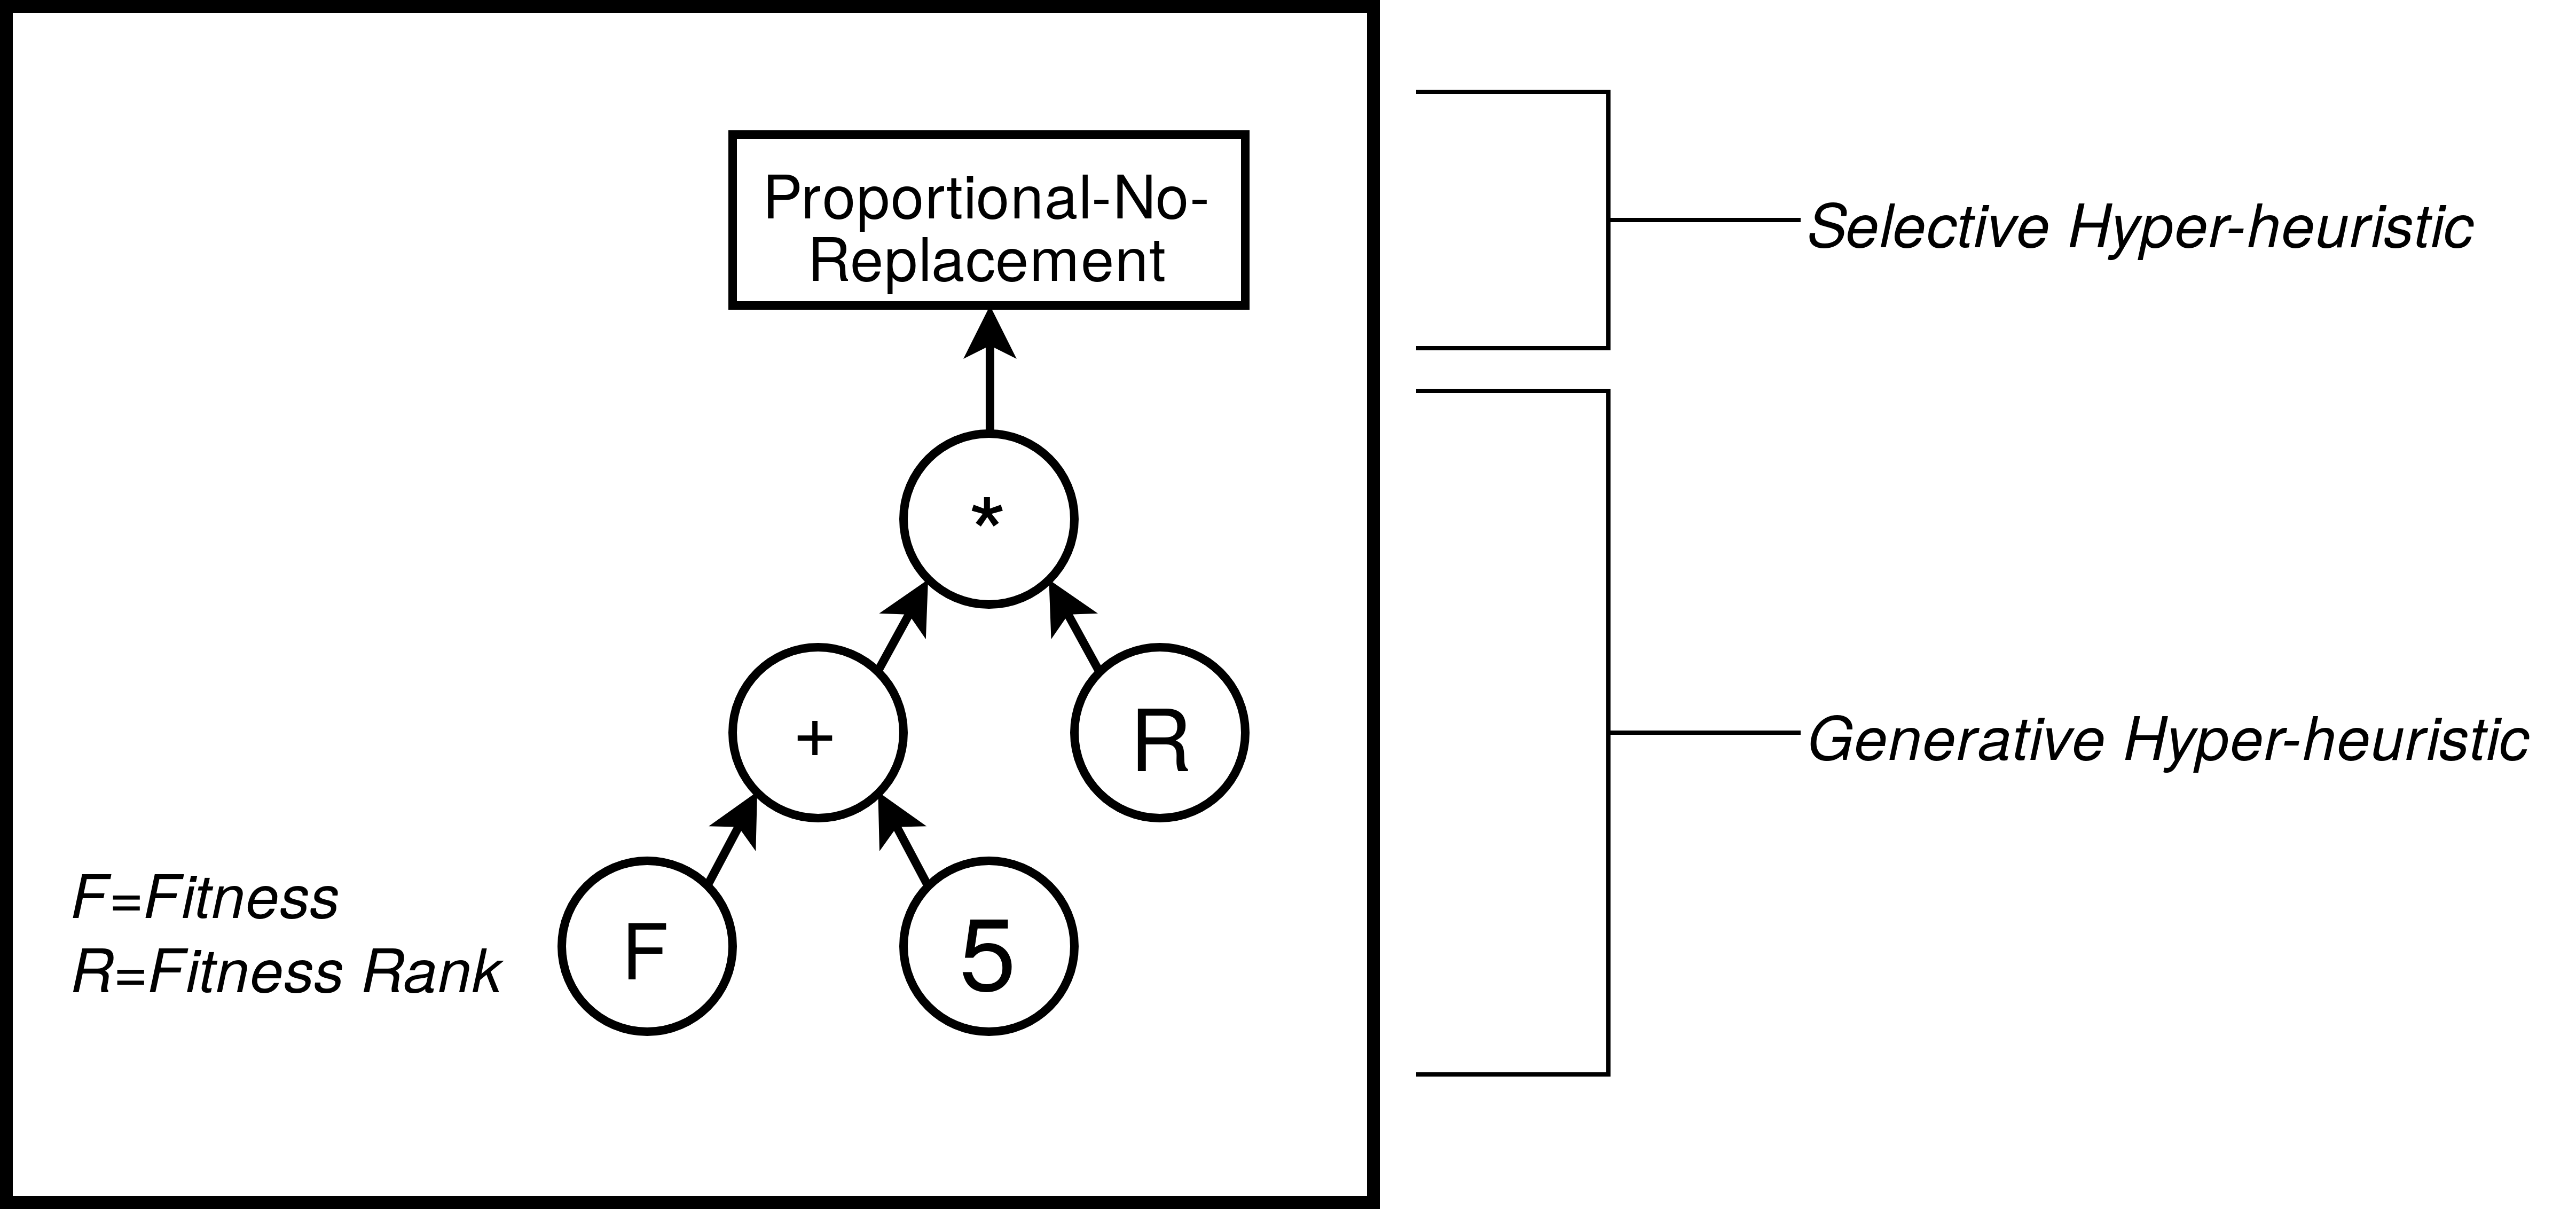
\includegraphics[width=0.9\textwidth]{example_eppsea}
    \caption{Example of a generated selection function.}
    \label{fig:example_adpsea}
\end{figure}

\begin{algorithm}
\caption{Probabilistic Selection Function}
\label{alg:ExampleSelection}
\begin{algorithmic}[1]
\Procedure {ExampleSelection}{$P$, $W$} \label{proc:ExampleSelection}
	\State $W \leftarrow 0,\forall p \in P$
	\ForAll {$p \in P$}
		\State $W(i) \leftarrow (p.Fitness + 5)*p.FitnessRank$
	\EndFor
	\State $w_{min} \leftarrow minimum(W)$	
	\State $s \leftarrow 0$
	\ForAll {$w \in W$}
		\If {$w_{min}  < 0$}
			\State $s \leftarrow s + (w - w_{min} )$			
		\Else
			\State $s \leftarrow s + w$		
		\EndIf	
	\EndFor
	\State $selected \leftarrow \emptyset$
	\For {$j \leftarrow 1,m$}
		\State{$r \leftarrow random(0,s)$}
		\State $i \leftarrow 1$
		\While {$r > W(i)$}
			\State $r \leftarrow r - W(i)$
			\State $i \leftarrow i + 1$
		\EndWhile	
		\State $selected \leftarrow selection \cup P(i)$
		\State $P \leftarrow P - P(i)$
	\EndFor
\EndProcedure
\end{algorithmic}
\end{algorithm}

\begin{figure}
    \centering
    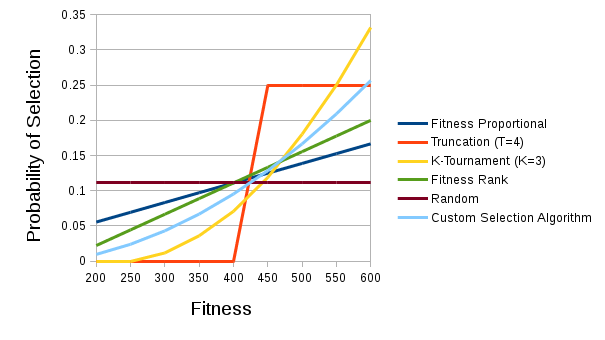
\includegraphics[width=0.99\textwidth]{selection_chances}
    \caption{A comparison of the chances that each member of a sample population, with fitnesses as listed, will be selected, under each of the typical selection strategies listed, as well as the custom selection strategy shown in Figure~\ref{fig:example_adpsea}.}
    \label{fig:selection_chances}
\end{figure}

\section{Search Methodology}
\label{Methodology-Search Methodology}

To develop high-quality selection functions, we need a method to search through the space of selection functions defined by the representation described in Section~\ref{Methodology-Encoding Selection Functions}. We use a meta-EA to develop the selection functions, treating each complete selection function as a member of a higher-order population. After generating an initial pool of randomly constructed selection functions, the quality of each selection function is determined, and well-performing selection functions are chosen to recombine and mutate into new candidate selection functions. 

The quality of each selection function is determined by running an underlying EA on a suite of static training instances from a benchmark problem class. The underlying EA utilizes the selection function in question, and keeps all other parameters constant. The performance of the underlying EA is averaged over multiple runs, and is used to determine the quality of a selection function; selection functions that enable the EA to perform better, with all other parameters constant, are considered to be ``higher-quality'' selection functions. This information is fed back into the meta-EA to generate the next set of candidate selection functions. Selection functions that perform extremely poorly, because they cause the EA to have either no selection pressure or negative selection pressure, are pruned out of the population and never used to generate new selection functions. To prevent the size of the GP-trees from growing too large, parsimony pressure is applied to the selection functions in the following manner; after the entire generation of selection functions is rated, the fitness assigned to each selection function is reduced by an amount equal to the number of nodes in all the function's GP-Trees, times a parsimony coefficient, times the difference in fitness between the best and worst selection functions in the population (after the extremely poor selection functions are removed).

When the meta-EA concludes, the bottom-level EA utilizing the best selection function from the meta-EA is run on a set of separate testing instances from the same problem class to test the generalization of the selection function's performance. If the EA utilizing the best selection function performs significantly better on the testing instances than the same EA using a standard selection function, then we can say that the evolved selection function successfully generalized to the problem class of interest.

The benchmark problem class used for the underlying EA are selected from two sources. The first source of benchmark problems is the MK-Landscape class of optimization problems \citep{whitley2016gray}. This problem set is a generalization of the NK-landscape problem class, first introduced in \citep{kaufmann1993origins}. This benchmark was chosen because the properties of the fitness landscape can be easily controlled with the N, M, and K parameters, as well as the policy with which the fitness values of the loci are generated. With one set of parameters, a wide range of new MK-Landscapes can be easily generated, making it easy to provide both a variety of training landscapes to tune a selection algorithm to, and a variety of new, separate landscapes to use for testing the generalization of the selection algorithm. 

As a second source of benchmark problems, we also select functions from the Comparing Continuous Optimizers (COCO) platform used for the GECCO Workshops on Real-Parameter Black-Box Optimization Benchmarking \citep{cocobbob}. This benchmark set provides a suite of real-valued optimization problems that serve as a robust testbed for optimization algorithms, including EAs. These problems are well-suited to measuring the strength of an EA and how well it performs under various conditions, which makes it an excellent choice for measuring how different selection functions impact the performance of an EA. Additionally, each problem class in the suite offers multiple problems, which allows us to both test the EA's performance on a variety of similar problems and test whether an increase in performance offered by a higher-quality selection function generalizes to other instances within the problem class.

\ThesisBodyChapter{Initial Experimentation}
\label{Initial Experimentation}
Here we discuss the initial experimentation performed with an earlier version of our Hyper-heuristic, to explore the prospects of using a Hyper-heuristic to evolve a relation between an individual's fitness score and the probability of being selected. The Hyper-heuristic used a methodology similar to the current version, as described in section \ref{Methodology-Encoding Selection Functions}. However, the GP operators were limited to the arithmetic functions (+, -, *, and /) and the step function. The GP terminals were limited to fitness, fitness ranking, population size, constant, and random. The selection methods were limited to proportional-replacement and proportional-no-replacement, so the GP-Tree always directly determined the relative probability that an individual was to be selected.

In the rest of this section, we briefly describe the experimental setup, as well as the observations resulting from this experiment, and how we incorporated this information into the current version of the Hyper-heuristic. For more details on the methodology and results of this experiment, refer to \citep{richter2018adpsea}, in which this work was originally published.

\section{Experimental Setup}
\label{Experimental Setup-Original}

We constructed a basic evolutionary algorithm, utilizing traditional parent selection, recombination, mutation, and survival selection. The target problem of the EA was an NK-Landscape problem \citep{whitley2016gray,kaufmann1993origins}. We used the Hyper-heuristic to evolve the parent selection stage of this EA. Survivor selection was always performed randomly, thus forcing the parent selection to provide all of the EA'se selection pressure. We evaluated selection functions by running the EA multiple times on each of a number of NK-Landscape functions, which are generated when the meta-EA is initialized and held constant throughout the experiment. The best fitnesses achieved by the population for each run of the EA using the selection function were averaged together and assigned to the selection function as its fitness at the Hyper-heuristic level. When the meta-EA terminates, the best selection function was tested against a number of conventional selection functions, including fitness proportional, truncation, and \textit{k}-tournament, with several values of \textit{k}. The NK-Landscape problems used for these tests were separately generated from the functions used during the meta-EA, to test generalization.

\section{Results, Observations, and Takeaways}
\label{Results-Original}

The evolved selection function significantly outperformed all of the conventional selections tested on 46 out of the 50 benchmark problems. This confirmed our initial hypothesis that, by using a Hyper-heuristic search through the space of selection functions as defined by our custom representation, a significant performance benefit can be achieved. However, for future experiments, we needed to show that an evolved selection function could not just outperform a number of handpicked selection functions, but the best possible selection function, with the best possible parameters, from our suite of conventional selection functions, in order to prove the validity of using our Hyper-heuristic versus conventional fitness tuning methods. Thus, for future experiments, we used automated parameter tuning to select the conventional selection function that the evolved selection function would be measured against. We also noted that our representation could only effectively represent a probabilistic selection scheme, which directly calculates the relative probability that an individual will be selected as a function of its fitness. Although it was possible to map other selection methodologies, such as tournament selection and truncation selection, to our custom representation (see Appendix \ref{apx:originalEppseaRepresentation} for examples of these mappings), such mappings were too complex to emerge during evolution, and so we built more options for the final selection method into the representation. With these new selection methods, we moved from evolving a GP-Tree to determine an individual's probability of selection, to evolving a GP-Tree that output a more general ``desirability'' score for an individual, and allowed various methods of selecting individuals based on their assigned desirability. We also sought more benchmark problem classes to test our methodology on, as we had only shown improvement and generalization for the NK-Landscape problem class. We additionally sought to tune selection for a more state-of-the-art method of evolutionary computing, as the EA for which we showed improvement was very basic.

The first of the three primary experiments presented in Section \ref{Primary Experiments} is an updated repetition of this experiment, with our updated methodology, on a problem class generalized from the NK-Landscape class. We describe this experiment in more detail in Section \ref{Evolution of Parent and Survival Selection For A Basic EA Solving MK-Landscapes}. The other two experiments incorporate the rest of our observations with new experimental setups.

\ThesisBodyChapter{Primary Experiments}
\label{Primary Experiments}

We conducted three sets of experiments with our meta-EA methodology. In our first experiment, we evolved new parent and survival selection functions for a basic evolutionary algorithm solving benchmark problems in the MK-Landscape problem class. This experiment is described further in Section \ref{Evolution of Parent and Survival Selection For A Basic EA Solving MK-Landscapes}.

In our second experiment, we used the same EA as in the first experiment, but instead solving for real-valued benchmark problems selected from the COCO platform. This experiment is described further in Section \ref{Evolution of Parent and Survival Selection For A Basic EA Solving Real-Valued Benchmarks}.

In our third experiment, we evolved a new mean-update scheme for a covariance matrix adaptation evolution strategy (CMA-ES) \cite{hansen1996cmaes}, solving from real-valued benchmark problems selected from the COCO platform. This experiment is described further in Section \ref{Evolution of Selection For CMA-ES Solving Real-Valued Benchmarks}.

The parameters for the meta-EA used in each experiment are shown in Table \ref{tab:Meta-EA Parameters}.

\begin{table}
\centering
  \caption{Meta-EA Parameters}
  \label{tab:Meta-EA Parameters}
  \begin{tabular}{cc}
    \toprule
    Parameter& Value\\
    \midrule
    Population Size & 40 \\
    \hline
    Offspring Size & 40\\
    \hline
    Evaluation Count & 4000\\
    \hline
    Max GP-Tree Initialization Depth & 4\\
    \hline
    Parent Selection & \textit{k}-tournament, \textit{k}=4 \\
    \hline
    Survival Selection & Truncation\\
    \hline
    Mutation & Subtree Regeneration\\
    \hline
    Crossover & Subtree Crossover\\
    \hline
    Parsimony Pressure Coefficient & 0.0005\\
    \hline
    Mutation Rate & 0.25\\
    \hline
    Range for Constant Terminals & [-100, 100]\\
    \hline
    Range for Random Terminals & [-100, 100]\\
    \hline
    Number of Runs (Training) & 5 \\
    \hline
    Number of Runs (Testing) & 200\\
    
  \bottomrule
\end{tabular}
\end{table}

\section{Evolution of Parent and Survival Selection For A Basic EA Solving MK-Landscapes}
\label{Evolution of Parent and Survival Selection For A Basic EA Solving MK-Landscapes}

Our first experiment is a repetition of our initial experiment described in section \ref{Initial Experimentation}, with the methodology described in Section \ref{Methodology} on a generalized problem class. For this experiment, we constructed a basic evolutionary algorithm, utilizing traditional parent selection, recombination, mutation, and survival selection. The target problem of the EA is an MK-Landscape problem, which is a generalization of the NK-Landscape problem \citep{whitley2016gray,kaufmann1993origins}. The EA has a number of parameters, including $\mu$, the population size; $\lambda$, the offspring size; parent and survival selection schemes; and a mutation rate. 

Each EA is assigned a single landscape to use when evaluating the population. When the EA is initialized, a set of $\mu$ random bitstrings is randomly generated as the initial population. The fitness of each bitstring is measured against the MK-Landscape. 2$\lambda$ individuals are selected from the population. The selected individuals are paired up, and one new individual is generated from each pair using per-bit crossover. The population of $\mu+lambda$ individuals is then culled back down to $\mu$ individuals using survival selection. The process repeats until the fitness of the population stops increasing, and the fitness of the best bitstring is taken as the final result of the EA run.

For the purposes of both determining the quality of evolved selection functions, and testing the generalization of their performance, a number of MK-Landscape problems are generated. Most of the generated problems are set aside for testing generalization, and the rest are used for training. Before the meta-EA is run, the optimal parameters for the EA are determined using the iRace parameter optimization package \citep{irace}. iRace is also used to determine schemes for traditional, non-evolved parent and survival selection, selecting from a number of typical parent and survival selection methods, such as truncation, fitness-proportional selection, and \textit{k}-tournament selection. For the purposes of determining these parameters with iRace, only the training problems are used, and not the testing problems. This way, we can compare the generalization of the selection functions picked by iRace to the generalization of the selection functions generated by the meta-EA.

Every member of the meta-EA population consists of two selection functions, which are evolved together as one genome. The first selection function is used for parent selection, and the second function is used for survival selection. When the meta-EA is initialized, each selection function in the initial meta-EA population is measured by running the underlying EA on each of the training problems, using the parameters found by iRace but substituting the evolved selection function for the iRace-picked selection schemes. The final result of the EA is averaged across all the training problems, for multiple runs per problem, and this mean is assigned as the fitness of the evolved selection function. Once all of the evolved selection functions have an assigned fitness, the meta-EA performs recombination and mutation to generate the next generation of selection functions, which are evaluated in the same way. The meta-EA continues until a number of generations pass with no improvement in the quality of the selection functions, at which point it terminates.

When the meta-EA terminates, the selection function with the highest fitness is selected, and EAs using this selection function are run on the testing problem instances. The EA is also run on the same testing instances using the original iRace parameters. The performance of the EA using the evolved selection function is then compared to the performance of the EA using the iRace-chosen selection methods to test for generalization.

Table \ref{tab:Bottom-level EA Parameters For MK-Landscape} shows the parameters used in the bottom-level EA and for generating the landscape functions. These parameters include the parent and survival selection functions chosen by iRace; for evaluating an evolved selection function, these functions are replaced with the evolved functions.

\begin{table} 
\centering
  \caption{Bottom-level EA Parameters For MK-Landscape}
  \label{tab:Bottom-level EA Parameters For MK-Landscape}
  \begin{tabular}{cc}
    \toprule
    Parameter & Value\\
    \midrule
    Population Size & 91 \\
    \hline
    Offspring Size & 34\\
    \hline
    Genome Length (N) & 40 \\
    \hline
    Locus Length (K) & 8\\
    \hline
    Number of Loci (M) & 40 \\
    \hline
    Locus Minimum Value & 0\\
    \hline
    Locus Maximum Value & 8\\
    \hline
    Parent Selection & Fitness Ranking With Replacement \\
    \hline
    Survival Selection & Fitness Ranking Without Replacement \\
    \hline
    Termination Criteria & Convergence \\
    \hline
    Generations to Convergence & 25\\
    \hline
    Mutation & Random Bit Flip \\
    \hline
    Mutation Rate & 0.0038\\
    \hline
    Crossover & Per-Bit Crossover\\
	
  \bottomrule
\end{tabular}
\end{table}

\section{Evolution of Parent and Survival Selection For A Basic EA Solving Real-Valued Benchmarks}
\label{Evolution of Parent and Survival Selection For A Basic EA Solving Real-Valued Benchmarks}

Our second experiment utilized a similar approach to our first experiment, but the benchmarks problem targeted by our EA were real-valued functions chosen from the 24 noiseless benchmark test functions contained in the COCO benchmark set. 

For each of the 24 problem classes, COCO offers multiple benchmark instances in each of several dimensionalities. For our experiment, we chose the 10-dimensional problems, and utilized all of the available instances for each of the 24 problem classes. For each of the problem classes, a number of the instances were chosen to be the training instances, used by the meta-EA to assign a fitness to an evolved selection function, and the rest of the instances were set aside as testing instances, to test for generalization.

As with the first experiment, each run of the underlying EA is initialized with a randomized population, but the population members are real-valued vectors initialized within a range recommended by COCO, rather than bitstrings. Parent selection, arithmetic recombination, mutation, and and survival selection are used to advance the EA until the population fitness is no longer increasing, and the best fitness attained by the EA is used as a measure of the EA's performance.

For this experiment, iRace was run for the training instances of each of the 24 problem classes individually, generating 24 sets of parameters for the EA. These parameters are listed in Appendix \ref{apx:iRaceBasicEACOCOParams}. 

The meta-EA was run as it was for the first experiment, with each evolved member containing two selection functions: one to replace parent selection, and one to replace survival selection. At the meta-EA's conclusion, the best selection function evolved is pitted against the traditional selection functions chosen by iRace, running on the testing problem instances to test generalization.

\section{Evolution of Selection For CMA-ES Solving Real-Valued Benchmarks}
\label{Evolution of Selection For CMA-ES Solving Real-Valued Benchmarks}

In the third experiment, we replaced the simple EA with a more complex covariance-matrix-adaptation evolution strategy (CMA-ES). This method repeatedly samples $\lambda$ points in a space around a mean, and uses a weighted combination of the high-value points to update the mean, as well as the parameters that control the shape of the space to be sampled in the next generation. In its traditional form, CMA-ES uses the $\mu$ highest-fitness points to update the mean; from an EA-perspective, this is akin to truncation selection.

For this experiment, we used the same meta-EA setup from previous experiments to evolve a new method of selecting which of the sampled points to use for recalculating the mean. Rather than selecting the $\mu$ highest-fitness points, the selection function selects a subset of all the sampled points, which are then ordered by fitness and used to update the mean. Once the mean is updated, all other state variables, such as the covariance matrix, are updated using the same methods as the unchanged CMA-ES.

To select benchmark functions, we tested the unmodified CMA-ES on the COCO functions. On many of the COCO functions, CMA-ES reaches close enough to the function's global optimum to meet the criteria set by COCO for solving the function. For each of the 24 function classes, we selected the lowest dimensionality for which CMA-ES was unable to find the global optimum (according to COCO's own criteria) at least half the time. We ignore the function classes for which CMA-ES is able to solve the instances more than half the time with $D\geq20$. The functions chosen are detailed in Table \ref{tab:experiment3chosenFunctions}. Unlike with the first two experiments, we did not use iRace to find a parameter set for CMA-ES before running the meta-EA, as CMA-ES is much less dependent on initial parameters. We use $lambda=10*D=100$, $\mu = \lambda/2 = 50$, and $\sigma_i = 0.5$. 

\begin{table}
\centering
  \caption{COCO Benchmark Functions Chosen For Experiment 3}
  \label{tab:experiment3chosenFunctions}
  \begin{tabular}{cc}
    \toprule
    Function Index & Dimensionality \\
    \midrule
    3 & 2\\
    \hline
    4& 2\\
    \hline
    6& 10\\
    \hline
    12& 10\\
    \hline
    15& 2\\
    \hline
    16& 10\\
    \hline
    19& 2\\
    \hline
    20& 2\\
    \hline
    21& 2\\
    \hline
    22& 2\\
    \hline
    23& 5\\
    \hline
    24& 2\\                        
	
  \bottomrule
\end{tabular}
\end{table}

When evaluating the performance of an evolved selection function to assign a fitness value to it, the fitness is taken as the proportion of the runs in which the modified CMA-ES reaches the global optimum, or moves close enough to it to meet the criteria to solve the problem.

\ThesisBodyChapter{Results}
\label{Results}
Here, we present the results observed from the three experiments performed.

\section{Results And Observations From First Experiment}
\label{firstExperimentResults}

For each of the problem instances in the testing set, we run the EA for 200 testing runs, both with the evolved selection functions and with the traditional selection functions. We then compare the final best fitnesses reached in the testing runs with a two-sided T-test to test for a significant difference. We found that, in 45 out of 50 of the testing instances, the EA using the evolved selection function reached a significantly higher final best fitness than the EA without one $(p=0.05)$. In the remaining 10 testing instances, there was no statistical difference between the EA with and without the evolved selection function.

Figure \ref{fig:experiment1Result} shows the parent selection stage of the best selection function evolved by the Hyper-heuristic. The survival selection was controlled by a separate, similar function.

\begin{figure}
    \centering
    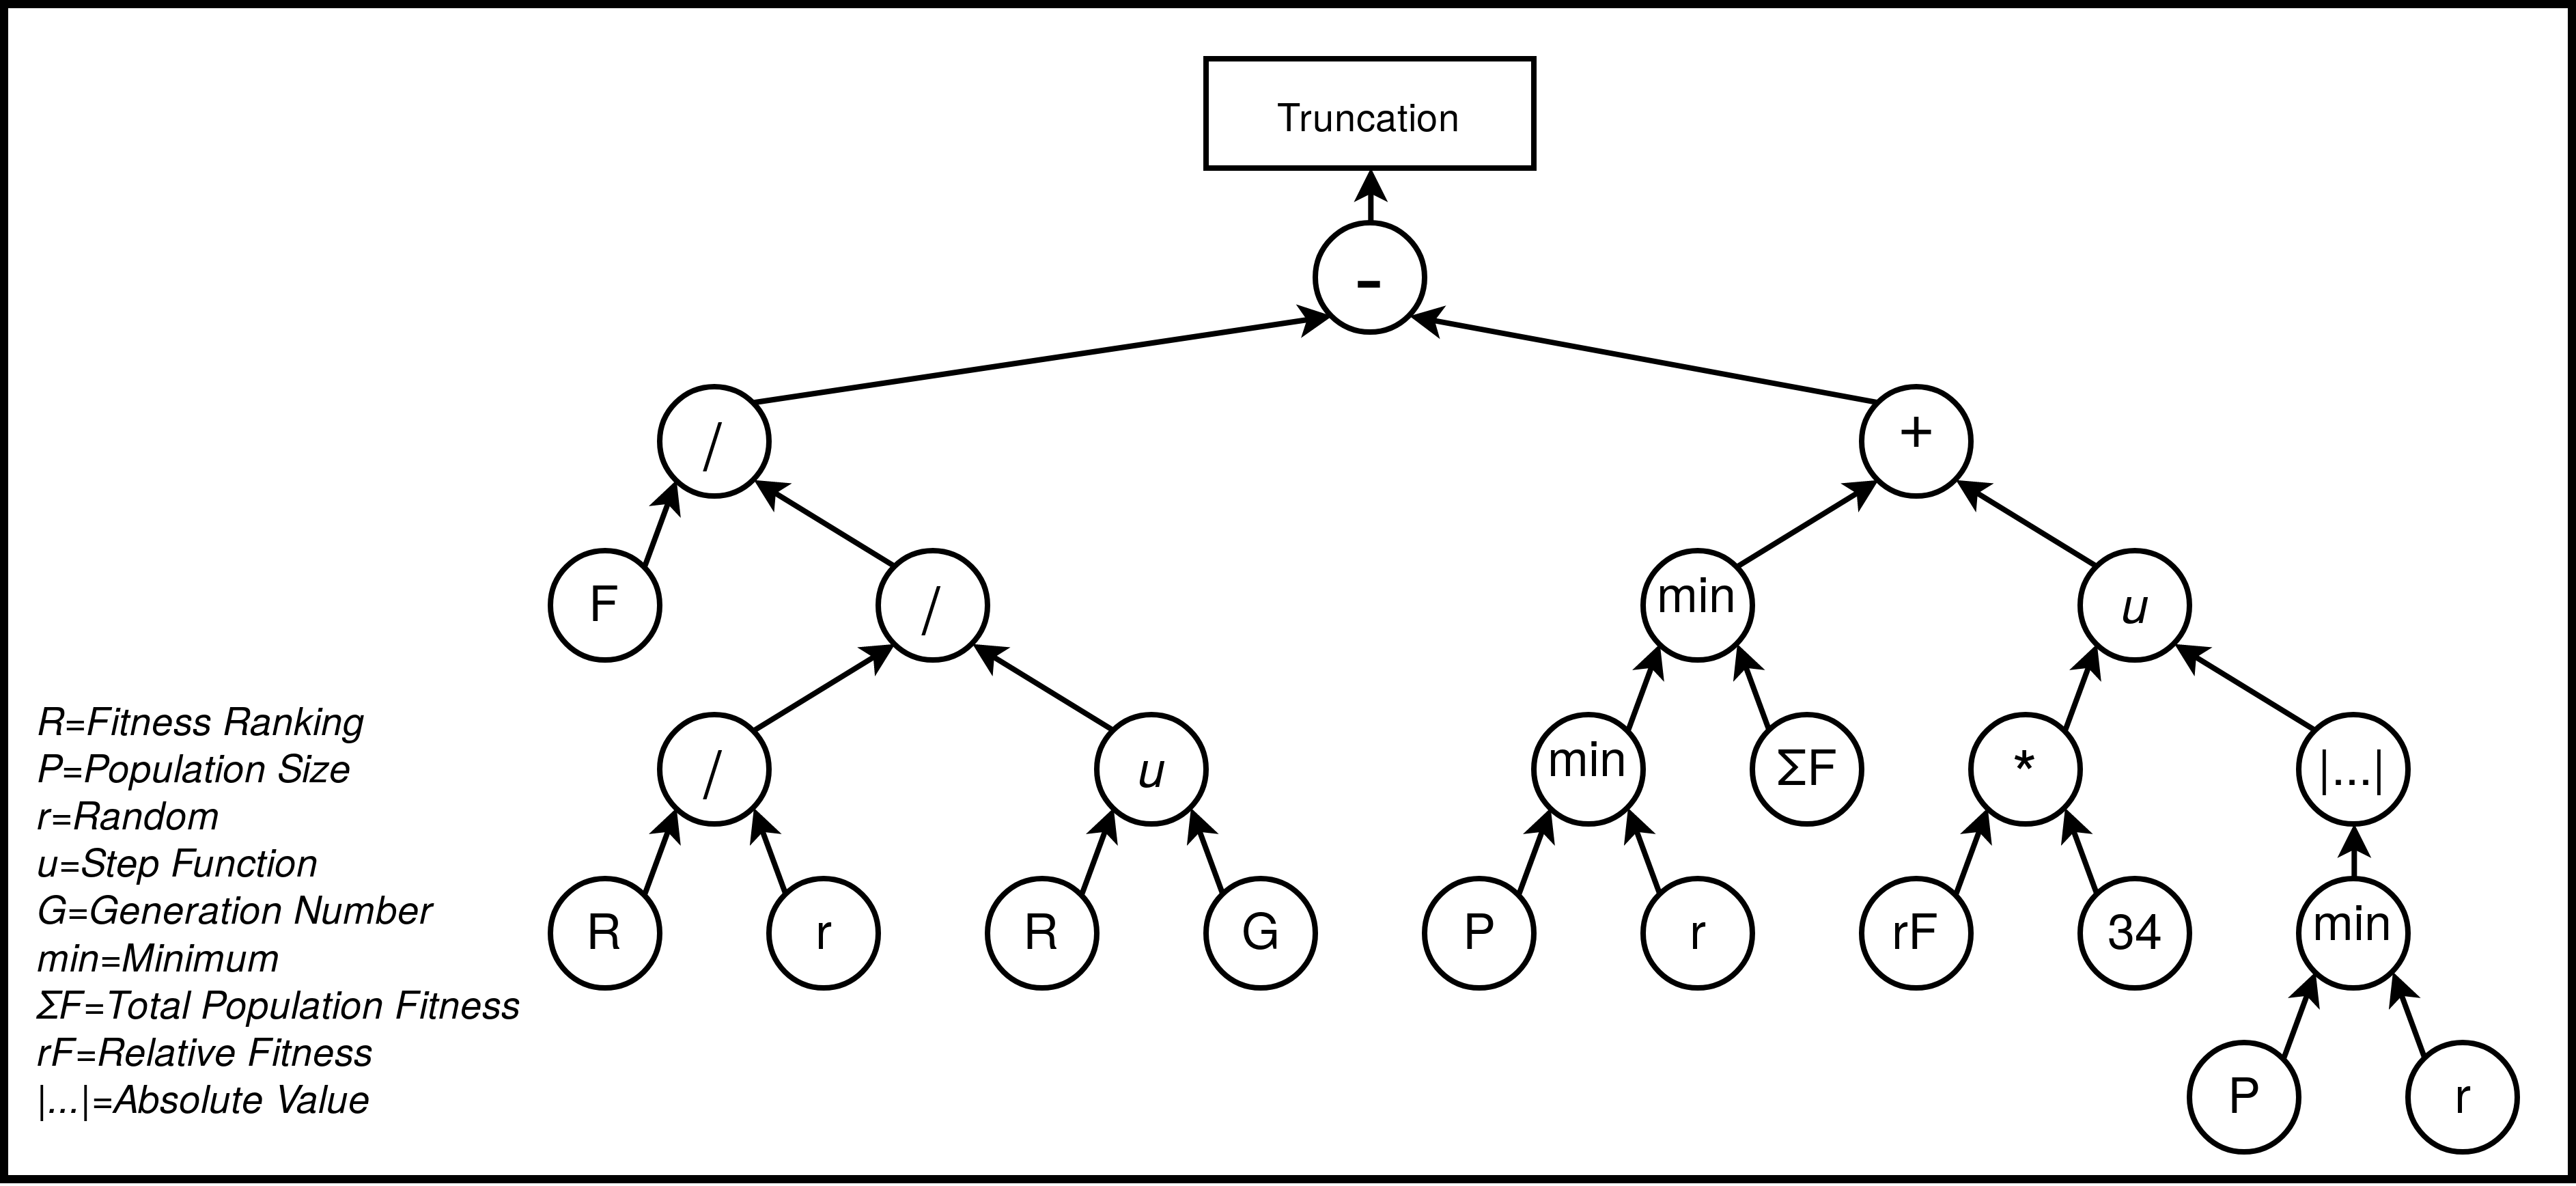
\includegraphics[width=0.9\textwidth]{experiment1Result}
    \caption{The function that controlled parent selection in the best evolved selection function.}
    \label{fig:experiment1Result}
\end{figure}

Figure \ref{fig:Experiment1LinePlot} shows the progression of the best population member's fitness through many runs of one of the testing functions, averaged for both the typical selection functions and he evolved selection functions. We see that, on average, the evolved selection function climbs more slowly towards a higher fitness before converging and terminating. Figure \ref{fig:Experiment1Boxplot} shows a boxplot comparison of the final best fitnesses achieved on the same testing fitness function, showing that, for this particular function, while the best fitnesses achieved by the evolved selection functions are generally within the same range as those found by the unmodified EA, they tend to be more consistently within the higher end, by comparison.

The general trend that we observe, across all the testing problems, is that the EA using the evolved selection functions tends to trend more slowly toward an area of high fitness than the EA using the traditional selection functions. Although the evolved selection functions take more evaluations to converge, they often converge at a higher fitness.
\begin{figure}
    \centering
    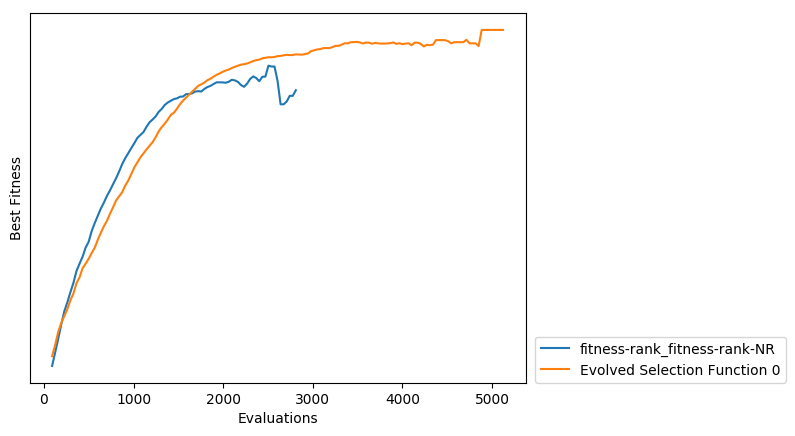
\includegraphics[width=0.9\textwidth]{Experiment1LinePlot}
    \caption{A plot of the best population fitness against the number of EA evaluations, achieved by both the typical selection function and the evolved selection function, averaged over all runs, for one of the testing functions.}
    \label{fig:Experiment1LinePlot}
\end{figure}

\begin{figure}
    \centering
    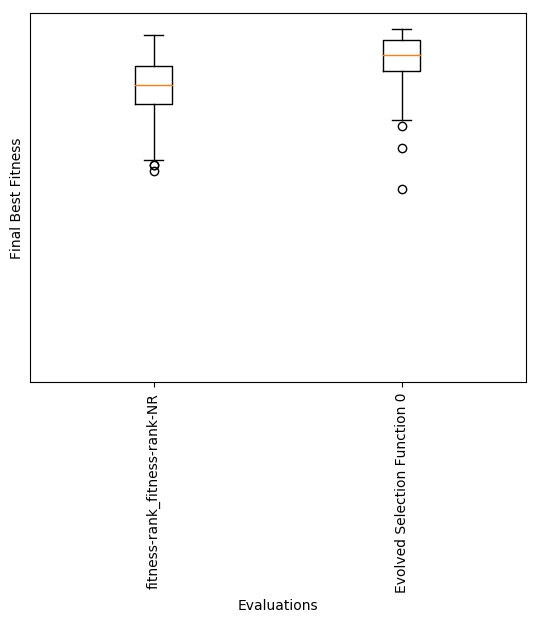
\includegraphics[width=0.9\textwidth]{Experiment1Boxplot}
    \caption{A box plot comparing the final best fitnesses achieved on one of the testing functions, by both the typical selection functions and the evolved selection functions.}
    \label{fig:Experiment1Boxplot}
\end{figure}

\section{Results And Observations From Second Experiment}
\label{secondExperimentResults}

For each of the problem instances in the testing set, we run the EA for 200 testing runs, both with the evolved selection functions and with the traditional selection functions. We then compare the final best fitnesses reached in the testing runs with a two-sided T-test to test for a significant difference. For each benchmark problem class in the COCO functions dataset, we count the number of instances for which we find a statistically significant difference between the final best fitness found by the EA with the best evolved selection function and the final best fitness found by the EA without one. These results are shown in Table \ref{tab:experiment2results}. 

\begin{table}
\centering
  \caption{Experiment 2 Results}
  \label{tab:experiment2results}
  \begin{tabular}{cc}
    \toprule
	Problem Index (D=10) & Number of Instances Improved \\
	\midrule
	F=1 & 0 / 12 \\
	\hline
	F=2 & 1 / 12 \\
	\hline
	F=3 & 2 / 12 \\
	\hline
	F=4 & 2 / 12 \\
	\hline
	F=5 & 5 / 12 \\
	\hline
	F=6 & 2 / 12 \\
	\hline
	F=7 & 7 / 12 \\
	\hline
	F=8 & 2 / 12 \\
	\hline
	F=9 & 12 / 12 \\
	\hline
	F=10 & 1 / 12 \\
	\hline
	F=11 & 7 / 12 \\
	\hline
	F=12 & 0 / 12 \\
	\hline
	F=13 & 2 / 12 \\
	\hline
	F=14 & 0 / 12 \\
	\hline
	F=15 & 0 / 12 \\
	\hline
	F=16 & 0 / 12 \\
	\hline
	F=17 & 4 / 12 \\
	\hline
	F=18 & 4 / 12 \\
	\hline
	F=19 & 12 / 12 \\
	\hline
	F=20 & 0 / 12 \\
	\hline
	F=21 & 8 / 12 \\
	\hline
	F=22 & 6 / 12 \\
	\hline
	F=23 & 0 / 12 \\
	\hline
	F=24 & 1 / 12 \\                       
	
  \bottomrule
\end{tabular}
\end{table}

We find that, for some problem classes, such as 7, 9, 11, 19, 21, and 22, the evolved selection function enabled the EA to perform significantly better in at least half of the testing instances used. For most of the testing cases, however, there were few or no testing instances for which the EA using the evolved selection function performed significantly better than the EA using only the parameters found by iRace. 

\section{Results And Observations From Third Experiment}
\label{thirdExperimentResults}

For each problem instance in the testing set, we run the CMA-ES for 200 testing runs, both using the evolved selection function and unmodified. We then measure, for each testing instance, the proportion of runs which solved the function, in each case. These results are shown in Table \ref{tab:experiment3Results}.

For the problem classes 4, 6, 12, 19, 20, and 21, the CMA-ES modified with the evolved selection function solved the problem instance more often than the unmodified CMA-ES. For the functions 4, 19, 20, and 21, the success rate of CMA-ES increased by 20-30 percent when modified with the evolved selection function. For functions 6 and 12, the effect is much more dramatic; on function 6, the success rate increased from 0 percent to around 96 percent, and on function 12, the success rate increased from 18-67 percent, varying across the function instances, to 100 percent for all function instances.

For the function indices 3, 15, 16, 23, and 24, there was no major difference between the success rate of the modified and unmodified CMA-ES.

\begin{table}
\centering
  \caption{Experiment 3 Results}
  \label{tab:experiment3Results}
  \begin{tabular}{ccccc}
    \toprule
	Problem Instance & F=3,D=2 & F=4,D=2 & F=6,D=10 & F=12,D=10\\
	\hline
	0 & 36.0\% / 34.5\% & 34.0\% / 4.0\% & 96.5\% / 0.0\% & 100.0\% / 41.0\%\\
	\hline
	1 & 32.5\% / 33.5\% & 36.0\% / 1.5\% & 96.0\% / 0.0\% & 100.0\% / 40.0\%\\
	\hline
	2 & 38.5\% / 38.0\% & 26.5\% / 2.0\% & 97.5\% / 0.0\% & 100.0\% / 55.5\%\\
	\hline
	3 & 37.5\% / 30.5\% & 34.5\% / 3.5\% & 94.5\% / 0.0\% & 100.0\% / 52.0\%\\
	\hline
	4 & 34.0\% / 35.0\% & 38.0\% / 3.5\% & 93.5\% / 0.0\% & 100.0\% / 51.5\%\\
	\hline
	5 & 35.0\% / 32.5\% & 9.0\% / 4.0\% & 95.0\% / 0.0\% & 100.0\% / 48.0\%\\
	\hline
	6 & 33.5\% / 35.0\% & 36.5\% / 4.5\% & 95.0\% / 0.0\% & 100.0\% / 18.0\%\\
	\hline
	7 & 38.0\% / 37.5\% & 37.5\% / 2.0\% & 98.0\% / 0.0\% & 100.0\% / 31.0\%\\
	\hline
	8 & 35.0\% / 33.5\% & 36.0\% / 3.5\% & 97.5\% / 0.0\% & 100.0\% / 36.0\%\\
	\hline
	9 & 36.5\% / 32.0\% & 33.5\% / 4.5\% & 96.5\% / 0.0\% & 100.0\% / 67.5\%\\
	\hline
	\hline
	Problem Instance & F=15,D=2 & F=16,D=10 & F=19,D=2 & F=20,D=2\\
	\hline
	0 & 40.0\% / 45.5\% & 39.5\% / 37.0\% & 48.0\% / 38.0\% & 45.0\% / 25.0\%\\
	\hline
	1 & 43.0\% / 47.0\% & 42.5\% / 41.5\% & 53.0\% / 38.0\% & 46.0\% / 22.5\%\\
	\hline
	2 & 47.0\% / 45.5\% & 40.0\% / 41.0\% & 58.0\% / 36.5\% & 54.0\% / 24.5\%\\
	\hline
	3 & 39.5\% / 40.0\% & 43.0\% / 38.5\% & 55.0\% / 30.0\% & 44.5\% / 22.5\%\\
	\hline
	4 & 40.0\% / 40.0\% & 42.0\% / 47.0\% & 54.0\% / 34.0\% & 46.0\% / 26.0\%\\
	\hline
	5 & 41.0\% / 45.0\% & 32.5\% / 38.0\% & 56.5\% / 40.0\% & 45.5\% / 26.5\%\\
	\hline
	6 & 38.0\% / 32.0\% & 45.5\% / 40.5\% & 55.5\% / 38.0\% & 50.0\% / 27.0\%\\
	\hline
	7 & 42.0\% / 42.5\% & 41.5\% / 42.0\% & 61.0\% / 32.0\% & 48.5\% / 23.5\%\\
	\hline
	8 & 43.0\% / 43.0\% & 37.5\% / 37.5\% & 53.0\% / 34.0\% & 54.5\% / 24.5\%\\
	\hline
	9 & 41.0\% / 39.0\% & 36.5\% / 34.0\% & 56.5\% / 40.5\% & 49.5\% / 26.0\%\\
	\hline
	\hline
	Problem Instance & F=21,D=2 & F=23,D=5 & F=24,D=2\\
	\hline
	0 & 61.0\% / 37.5\% & 25.0\% / 39.0\% & 1.0\% / 3.0\%& \\
	\hline
	1 & 36.0\% / 19.5\% & 26.5\% / 28.0\% & 0.5\% / 1.0\%& \\
	\hline
	2 & 59.5\% / 28.0\% & 29.5\% / 30.0\% & 0.5\% / 1.5\%& \\
	\hline
	3 & 66.5\% / 37.0\% & 37.5\% / 35.0\% & 3.5\% / 1.0\%& \\
	\hline
	4 & 38.5\% / 18.5\% & 31.5\% / 29.0\% & 2.5\% / 0.5\%& \\
	\hline
	5 & 34.5\% / 16.5\% & 30.0\% / 33.0\% & 1.0\% / 2.0\%& \\
	\hline
	6 & 63.0\% / 24.5\% & 33.0\% / 33.5\% & 1.0\% / 0.5\%& \\
	\hline
	7 & 56.0\% / 28.5\% & 35.5\% / 30.0\% & 3.5\% / 2.0\%& \\
	\hline
	8 & 76.5\% / 33.0\% & 35.5\% / 26.5\% & 1.0\% / 2.0\%& \\
	\hline
	9 & 76.5\% / 33.5\% & 36.5\% / 28.0\% & 1.5\% / 1.0\%& \\
	
  \bottomrule
\end{tabular}
\end{table}
 
\ThesisBodyChapter{Conclusions}
\label{Conclusion}
We hypothesized that a Hyper-heuristic search through the space of selection functions for EAs could improve the performance of an EA on a particular problem class by discovering a specialized selection function. We developed a representation of selection functions that uses a Koza-style GP-Tree to relate an individual's fitness value and fitness ranking to its relative probability of selection, and used a meta-EA to search through the space of selection functions in this representation. 

In our first experiment, we observed that, for an EA with a given set of parameters, an evolved selection function can lead to a significant increase in performance that successfully generalizes to other similar instances in the same problem class. The behavior that we see in the EAs using the evolved selection functions, where the fitness grows more slowly and converges later, at a higher fitness, suggests that the meta-EA evolved toward selection schemes with less selection pressure on the population, allowing them to explore further to find better optima. Even though the candidate parameters for the EA, as selected by iRace, included several selections of varying selection pressures (including \textit{k}-tournament with configurable \textit{k}), the evolved selection functions still seemed to find a better balance of exploration vs. exploitation.

In our second experiment, we observed varying results in the ability for the EA with the evolved selection function to outperform the EA without one. In some cases, a large improvement was seen by applying the evolved selection function, resulting in the EA finding significantly higher fitnesses in at least half the testing instnaces. In many cases, applying the evolved selection function results in significantly higher fitnesses on fewer than half of the test cases, and in some cases, there is no observed significant improvement whatsoever. This deficiency could be due to a number of factors. It is possible that, within the meta-EA, the evolved selection functions over-specialized to the training functions provided, and sacrificed the ability to generalize for increased improvement on the training functions. It is also possible that some of the functions selected from the COCO benchmarks are sufficiently complex that the EA setup we used required a more sophisticated improvement than a new selection function to gain an appreciable benefit to solving these functions. Some functions chosen may also be so simple that the EA already performs well enough that a change in selection function has a negligible impact on performance, as long as it exerts sufficient selection pressure. We attempted to remedy the issue of function difficulty in our third experiment by carefully selecting functions for which the unmodified CMA-ES performed moderately, but not exceptionally, well.

For our third experiment, we observed that evolving a new selection function for CMA-ES increased its solution on 6 of the 11 functions tested. In particular, we observed two cases with high dramatic improvements: the tests for COCO function classes 6 and 12. In the case of function class 6, the unmodified CMA-ES was unable to solve any of the testing instances, but the CMA-ES using the evolved selection solved these instances nearly 100\% of the time. In the case of function class 12, the success rate of the unmodified CMA-ES varied strongly between instances, ranging from 18 to 67\%. The modified CMA-ES, however, solved every test instance, reaching the global best fitness in each of 200 runs, on each of the testing instances, achieving a 100\% success rate. By observing the increases in success rate for some of the functions, it is clear that evolving a new selection scheme for CMA-ES provides a substantial benefit in some cases. The five cases where no improvement was observed involved functions that were highly multimodal. Three of these function were variants of the Rastrigin function, a highly multimodal function and the other two---the Weierstrass Function and the Katsuura Function---are highly rugged. It is likely, in these cases, that CMA-ES requires some other improvement aside from a new selection scheme to better learn and traverse the global structures of these functions. Because we only replaced the selection scheme of CMA-ES, we only changed how it internally updates the mean. Improving the performance of CMA-ES on these functions likely requires more intelligent updating of the other internal variables of CMA-ES, such as the evolution paths, the covariance matrix, and the step size.

We have shown that, with a meta-EA, it is possible to generate new selection functions, tuned to a particular benchmark problem, that can enable an EA to significantly outperform conventional selection functions on those problems. Thus, we show that, in order to discover the optimum selection method for an EA operating on a particular problem, it may not be sufficient to use any of the static conventional selection functions tested. We have also shown that, in some cases, this performance increase from a custom selection algorithm will generalize to similar problems in the same problem class. Therefore, if one expects to run the same EA on many problems from the same problem class, one might expect to gain a performance increase by doing some \textit{a priori} calculation to develop a specialized selection algorithm trained on instances of that problem class, which would then enable an EA utilizing that selection function to perform better on other instances of that problem class. However, our experiments have also shown that, for certain functions, replacing only the selection function may not yield significant performance improvements, depending on the behavior of the search strategy and the nature of the function being optimized by the EA. Careful consideration must be done to determine what the effect of tuning the selection scheme of a given EA will be on the performance of that EA, and whether such tuning will cause the EA to have an appreciable performance increase on the problem class in question. 

\ThesisBodyChapter{Threats To Validity}
\label{Threats to Validity}
Although we strove to ensure the robustness of our methodology and experimental setup, there are some careful considerations that must be made when interpreting these results which may threaten the validity of our claims.

Of obvious note is the fact that, while we have shown improved performance on the benchmark functions tested, we still have yet to test this method on EAs run in real-world scenarios, and we do not yet know whether the supposed performance benefit is, in practice, enough to warrant the \textit{a priori} computation necessitated by our methods.

In experiments 1 and 2, we used a very rudimentary EA, and it is highly unlikely that such an EA would be the best practical approach for a given problem, given the countless advancements in the field of evolutionary computing. We chose such a simple EA to illustrate our point that the selection function, while deceptively simple to configure by selecting a conventional selection function with proven effectiveness, has a large impact on the performance of an EA.

For our third experiment, we chose CMA-ES as a testing target for extending our method to a more state-of-the-art method. However, the implementation of CMA-ES we used was fairly basic, lacking restarts in particular, and much research has been done on improved and alternative variants of CMA-ES. For certain problems, these newer variants may offer the same, or greater, performance increases as an evolved selection function. However, if these newer variants also use some selection function to update internal variables, as the basic implementation does, then evolving a new selection function for these newer variants could generate an even greater increase in performance; this opens up an avenue for future research.

Some of the terminals used by the GP-Trees enable selection functions to have access to some information that conventional selection functions such as fitness proportional selection and truncation selection do not have. This information includes generation number and genome uniqueness, which can allow the selection function to account for other factors besides the fitness of the individual and the population at large. This might make the comparison to these functions in experiments 1 and 2 unfair. We chose the set of conventional selection functions available to iRace in experiments 1 and 2 as the functions that are commonly used in straightfoward EAs, in order to show that an evolved selection function with access to additional information may be worth the \textit{a priori} computation cost if the alternative is to simply use a simpler, conventional selection function selected from the most common choices that would work acceptably well for most EAs.



\ThesisBodyChapter{Future Work}
The work presented in this paper opens a number of potential avenues for future research. Of primary concern is the fact that the meta-EA presented in this paper requires a large amount of \textit{a priori} computation to generate a high-quality selection function. While this computational cost may be worth it for EAs that will run on problems from the same problem class many times, a more efficient method of finding good selection functions has a much greater potential to benefit EAs in general. 

The EA and CMA-ES in our experiments were tuned to increase performance on the MK-Landscape problem class and the COCO benchmark problem classes. While these problems are difficult and non-trivial to optimize for, they are entirely artificial, and the meta-EA has not yet been used to tune an EA for solving a real-world problem class. While the MK-Landscape problem class and related problems are used in several real-world fields, a major next step for this work is to apply the meta-EA to real-world EAs that could benefit from new, specialized selection functions. Of particular interest are EAs that are expected to be run many times on problems from the same general problem class, which would, over many runs, amortize the \textit{a priori} calculation required to tune the selection function.

Because the objective of this paper is similar to the work done to develop selection algorithms via Grammatical Evolution, it remains to be seen which cases each method is more effective for, and a direct comparison of the two methods on the same benchmark problem may yield more insight into which offers better performance benefits under certain conditions.

In the case of Experiments 1 and 2, the evolved selection functions were only tested against basic selection functions that lacked any self-adaptability. More work will need to be done to determine whether the best evolved selection functions can stand up to more dynamic, adaptable selection methods, if EAs such as the one used in Experiments 1 and 2 are targeted for improvement.

For the third experiment, the framework of CMA-ES used was fairly basic, lacking features such as restarts. In addition, many techniques have been developed to improve the performance of CMA-ES on functions where it may be deficient. Evolving a specialized selection function for these new forms of CMA-ES may lead to even greater performance gains, or may not even be necessary for particular problem classes. Additionally, as we noted in our conclusions, we only made efforts to improve the selection of points used in the mean-update step of CMA-ES, which allowed to it gain increased performance in some, but not all, of the problem cases tested. Further experiments to tune the selection of points used for updating the other internal variables, such as evolution path, covariance matrix, and step-size, may lead to greater changes in the behavior of CMA-ES, and thus, greater changes in performance.

For our meta-EA, the GP-Trees utilized several terminals related to the individual, such as fitness, fitness ranking, uniqueness of genome, and birth generation, as well as terminals related to the evolution at large, such as population size and generation number. Adding additional available terminals increases the information available to the meta-EA, allowing it to potentially evolve more intelligent selection functions. In particular, there are no terminals that allow the selection function to have any internal memory from generation to generation, such as the best fitness of past generations or which individuals have been selected previously. Additionally for EA's with sexual reproduction, or selection schemes involving individuals selected in pairs or groups, there is no terminal that measures two individuals relative to each other. This prevents the meta-EA from developing a selection function based on any information about an individual's mate, such as fitness, genome, etc. To add these terminals to the meta-EA, the selection function representation would need to be updated such that, when determining the desirability of an individual, the GP-Tree would take as input the information of some other individual to be selected for a similar purpose, such as recombination of the same child (for an EA with two-parent recombination) or selection for update of the same internal variable (for an Evolution Strategy such as CMA-ES).

\end{ThesisBody}




 % ... appendix - specify number of appendix chapters ...

\begin{ThesisAppendix}{two}{false}{false}


\ThesisAppendixChapter{Psuedocode For Final Selection Methods}
\label{apx:SelectionPsuedocode}

Here, we provide psuedocode to describe the procedures of the final selection methods utilized by the evolved selection functions. Refer to table \ref{tab:selection_methods} for a list and description of the selection methods. Note that each of these methods take, as input, a population \textit{P} of length \textit{n}, from which individuals will be selected; a number of individuals \textit{m} to be selected; and a function \textit{F}, which is the mathematical function encoded by the GP-Tree associated with the selection function. The method returns a list of the selected individuals. \textit{F} takes, as input, the population \textit{P}, and a population member \textit{p}, and returns a real number, representing the desirability score of the population member.

Algorithm \ref{alg:ProportionalReplacement} describes the procedure for Proportional-Replacement selection.

\begin{algorithm}
\caption{Proportional Selection With Replacement}
\label{alg:ProportionalReplacement}
\begin{algorithmic}[1]
\Procedure {ProportionalReplacement}{$P$, $m$, $F$} \label{proc:ProportionalReplacement}
	\State $W \leftarrow 0,\forall p \in P$
	\ForAll {$p \in P$}
		\State $W(i) \leftarrow F(P,p)$
	\EndFor
	\State $w_{min} \leftarrow minimum(W)$	
	\State $s \leftarrow 0$
	\ForAll {$w \in W$}
		\If {$w_{min}  < 0$}
			\State $s \leftarrow s + (w - w_{min} )$			
		\Else
			\State $s \leftarrow s + w$		
		\EndIf	
	\EndFor
	\State $selected \leftarrow \emptyset$
	\For {$j \leftarrow 1,m$}
		\State{$r \leftarrow random(0,s)$}
		\State $i \leftarrow 1$
		\While {$r > W(i)$}
			\State $r \leftarrow r - W(i)$
			\State $i \leftarrow i + 1$
		\EndWhile	
		\State $selected \leftarrow selection \cup P(i)$
	\EndFor
\EndProcedure
\end{algorithmic}
\end{algorithm}

Algorithm \ref{alg:ProportionalNoReplacement} describes the procedure for Proportional-No-Replacement selection.

\begin{algorithm}
\caption{Proportional Selection Without Replacement}
\label{alg:ProportionalNoReplacement}
\begin{algorithmic}[1]
\Procedure {ProportionalReplacement}{$P$, $m$, $F$} \label{proc:ProportionalNoReplacement}
	\State $W \leftarrow 0,\forall p \in P$
	\ForAll {$p \in P$}
		\State $W(i) \leftarrow F(P,p)$
	\EndFor
	\State $w_{min} \leftarrow minimum(W)$	
	\State $s \leftarrow 0$
	\ForAll {$w \in W$}
		\If {$w_{min}  < 0$}
			\State $s \leftarrow s + (w - w_{min} )$			
		\Else
			\State $s \leftarrow s + w$		
		\EndIf	
	\EndFor
	\State $selected \leftarrow \emptyset$
	\For {$j \leftarrow 1,m$}
		\State{$r \leftarrow random(0,s)$}
		\State $i \leftarrow 1$
		\While {$r > W(i)$}
			\State $r \leftarrow r - W(i)$
			\State $i \leftarrow i + 1$
		\EndWhile	
		\State $selected \leftarrow selection \cup P(i)$
		\State $P \leftarrow P - P(i)$
	\EndFor
\EndProcedure
\end{algorithmic}
\end{algorithm}

Algorithm \ref{alg:TournamentReplacement} describes the procedure for \textit{k}-Tournament-Replacement selection. Note the additional parameter \textit{k}, which controls the size of the tournaments.

\begin{algorithm}
\caption{\textit{k}-Tournament Selection With Replacement}
\label{alg:TournamentReplacement}
\begin{algorithmic}[1]
\Procedure {ProportionalReplacement}{$P$, $m$, $F$, $k$} \label{proc:TournamentReplacement}
	\State $selected \leftarrow \emptyset$
	\For {$j \leftarrow 1,m$}
		\State $tournament \leftarrow k$ members selected randomly from $P$
		\State $MaxScore = -\inf$

		\ForAll {$t \in tournament$}
			\If {$F(P,p) > MaxScore$}
				\State {$winner \leftarrow p$}
				\State {$MaxScore \leftarrow F(P,p)$}
			\EndIf			
		\EndFor
		\State $selected \leftarrow selection \cup p$
	\EndFor
\EndProcedure
\end{algorithmic}
\end{algorithm}

Algorithm \ref{alg:TournamentNoReplacement} describes the procedure for \textit{k}-Tournament-No-Replacement selection. Note the additional parameter \textit{k}, which controls the size of the tournaments.

\begin{algorithm}
\caption{\textit{k}-Tournament Selection Without Replacement}
\label{alg:TournamentNoReplacement}
\begin{algorithmic}[1]
\Procedure {ProportionalReplacement}{$P$, $m$, $F$, $k$} \label{proc:TournamentNoReplacement}
	\State $selected \leftarrow \emptyset$
	\For {$j \leftarrow 1,m$}
		\State $tournament \leftarrow k$ members selected randomly from $P$
		\State $MaxScore = -\inf$

		\ForAll {$t \in tournament$}
			\If {$F(P,p) > MaxScore$}
				\State {$winner \leftarrow p$}
				\State {$MaxScore \leftarrow F(P,p)$}
			\EndIf			
		\EndFor
		\State $selected \leftarrow selection \cup p$
		\State $P \leftarrow P - p$
	\EndFor
\EndProcedure
\end{algorithmic}
\end{algorithm}

Algorithm \ref{alg:Truncation} describes the procedure for Truncation selection.

\begin{algorithm}
\caption{Truncation}
\label{alg:Truncation}
\begin{algorithmic}[1]
\Procedure {ProportionalReplacement}{$P$, $m$, $F$} \label{proc:Truncation}
	\State $W \leftarrow 0,\forall p \in P$
	\ForAll {$p \in P$}
		\State {$W(i) \leftarrow F(P,p)$}
	\EndFor
	\State {$P \leftarrow P$ sorted by $W$, descending}
	\State {$selected \leftarrow \emptyset$}
	\For {$j \leftarrow 1,m$}
		\State $selected \leftarrow selection \cup P(j)$
	\EndFor
\EndProcedure
\end{algorithmic}
\end{algorithm}

Algorithm \ref{alg:SUS} describes the procedure for Stochastic-Universal-Sampling selection.

\begin{algorithm}
\caption{Proportional Selection With Replacement}
\label{alg:SUS}
\begin{algorithmic}[1]
\Procedure {ProportionalReplacement}{$P$, $m$, $F$} \label{proc:SUS}
	\State $W \leftarrow 0,\forall p \in P$
	\ForAll {$p \in P$}
		\State $W(i) \leftarrow F(P,p)$
	\EndFor
	\State $w_{min} \leftarrow minimum(W)$	
	\State $s \leftarrow 0$
	\ForAll {$w \in W$}
		\If {$w_{min}  < 0$}
			\State $s \leftarrow s + (w - w_{min} )$			
		\Else
			\State $s \leftarrow s + w$		
		\EndIf	
	\EndFor
	\State $selected \leftarrow \emptyset$
	\State $interval \leftarrow s / n$
	\State $offset \leftarrow random(0,interval)$
	\For {$j \leftarrow 1,m$}
		\State{$r \leftarrow (j-1)*interval + offset$}
		\State $i \leftarrow 1$
		\While {$r > W(i)$}
			\State $r \leftarrow r - W(i)$
			\State $i \leftarrow i + 1$
		\EndWhile	
		\State $selected \leftarrow selection \cup P(i)$	
	\EndFor
\EndProcedure
\end{algorithmic}
\end{algorithm}

\ThesisAppendixChapter{iRace Generated EA Parameters For Basic EA Running On Real-Valued Problems}
\label{apx:iRaceBasicEACOCOParams}

For each of the 24 benchmark functions in the COCO benchmark set, a set of optimal parameters for the EA was found using the iRace tuning package. The parameters used are listed here, in Table \ref{tab:iRaceBasicEAParams}. The parent and survival selection schemes are also tuned, and these selections are shown in Table \ref{tab:iRaceBasicEASelection}. Note that, during the meta-EA, these parent and survival selection are replaced by the evolved parent and survival selection schemes, and are only used when testing against the final evolved selection function at the end of the meta-EA. 

\begin{table}
\centering
  \caption{iRace tuned parameters for EA used in Experiment 2}
  \label{tab:iRaceBasicEAParams}
  \begin{tabular}{cccc}
    \toprule
    Function Index & Population Size & Offspring Size & Mutation Rate\\
    \midrule
	1 & 54 & 99 & 0.1021\\
	\hline
	2 & 15 & 96 & 0.1172\\
	\hline
	3 & 45 & 82 & 0.0853\\
	\hline
	4 & 28 & 96 & 0.1576\\
	\hline
	5 & 3 & 89 & 0.8467\\
	\hline
	6 & 4 & 86 & 0.3399\\
	\hline
	7 & 13 & 93 & 0.3261\\
	\hline
	8 & 10 & 98 & 0.1403\\
	\hline
	9 & 18 & 73 & 0.0893\\
	\hline
	10 & 23 & 76 & 0.2451\\
	\hline
	11 & 15 & 75 & 0.1801\\
	\hline
	12 & 55 & 96 & 0.0914\\
	\hline
	13 & 88 & 95 & 0.1656\\
	\hline
	14 & 13 & 96 & 0.1963\\
	\hline
	15 & 62 & 99 & 0.0066\\
	\hline
	16 & 89 & 81 & 0.157\\
	\hline
	17 & 85 & 97 & 0.1521\\
	\hline
	18 & 43 & 92 & 0.1178\\
	\hline
	19 & 33 & 93 & 0.1141\\
	\hline
	20 & 31 & 91 & 0.1748\\
	\hline
	21 & 42 & 97 & 0.3282\\
	\hline
	22 & 89 & 84 & 0.1373\\
	\hline
	23 & 16 & 92 & 0.1704\\
	\hline
	24 & 20 & 80 & 0.053\\              
		
  \bottomrule
\end{tabular}
\end{table}

\begin{table}
\centering
\caption{iRace tuned selection functions for EA used in Experiment 2. Tournament, proportional, and ranking selections are performed with replacement, except where otherwise noted.}
\label{tab:iRaceBasicEASelection}
  \begin{tabular}{cp{5cm}p{5cm}}
	\toprule
    Function Index & Parent Selection & Survival Selection \\
    \midrule
	1 & \textit{k}-tournament, \textit{k}=15 & \textit{k}-tournament without replacement, \textit{k}=89  \\ 
	\hline
	2 & Fitness ranking & truncation\\
	\hline
	3 & \textit{k}-tournament , \textit{k}=15 & Truncation \\ 
	\hline
	4 & \textit{k}-tournament , \textit{k}=12 & Truncation \\ 
	\hline
	5 & Stochastic Universal Sampling & Truncation\\
	\hline
	6 & Fitness ranking & Truncation  \\ 
	\hline
	7 & Fitness ranking & Truncation   \\ 
	\hline
	8 & Fitness ranking & Truncation   \\ 
	\hline
	9 & Fitness proportional & Truncation   \\ 
	\hline
	10 & Fitness proportional & Truncation   \\ 
	\hline
	11 & Fitness proportional & Truncation   \\    \\ 
	\hline
	12 & \textit{k}-tournament, \textit{k}=16 & Truncation   \\ 
	\hline
	13 & \textit{k}-tournament, \textit{k}=51 & Truncation    \\ 
	\hline
	14 & Fitness ranking & \textit{k}-tournament without replacement, \textit{k}=40   \\ 
	\hline
	15 & Fitness ranking & Truncation   \\ 
	\hline
	16 &  \textit{k}-tournament, \textit{k}=18 & Truncation  \\ 
	\hline
	17 &  \textit{k}-tournament, \textit{k}=12 & Truncation  \\ 
	\hline
	18 &  Fitness ranking & Truncation  \\ 
	\hline
	19 &  Fitness ranking & \textit{k}-tournament without replacement, \textit{k}=30  \\ 
	\hline
	20 &  \textit{k}-tournament, \textit{k}=15 & Truncation   \\ 
	\hline
	21 &  Fitness ranking & Truncation  \\ 
	\hline
	22 &  \textit{k}-tournament, \textit{k}=37 & Truncation  \\ 
	\hline
	23 &  Fitness ranking & Truncation  \\ 
	\hline
	24 &  Fitness ranking & Truncation  \\ 
	
	\bottomrule      
\end{tabular}
\end{table}




\ThesisAppendixChapter{Representations of Conventional Selection Functions in Initial Experimentation}
\label{apx:originalEppseaRepresentation}

In the earlier version of our selection function representation, as presented in \citep{richter2018adpsea}, the GP-Trees were used to directly evolved the relative probability that an individual would be selected, as a function of its fitness, fitness ranking, and population size. This method closely resembles fitness proportional selection, but other selection schemes can be represented in this format as well. In Figure \ref{fig:old_eppsea_representation}, we show how examples of these selection schemes would be represented by the evolved GP-Tree.

\begin{figure}
    \centering
    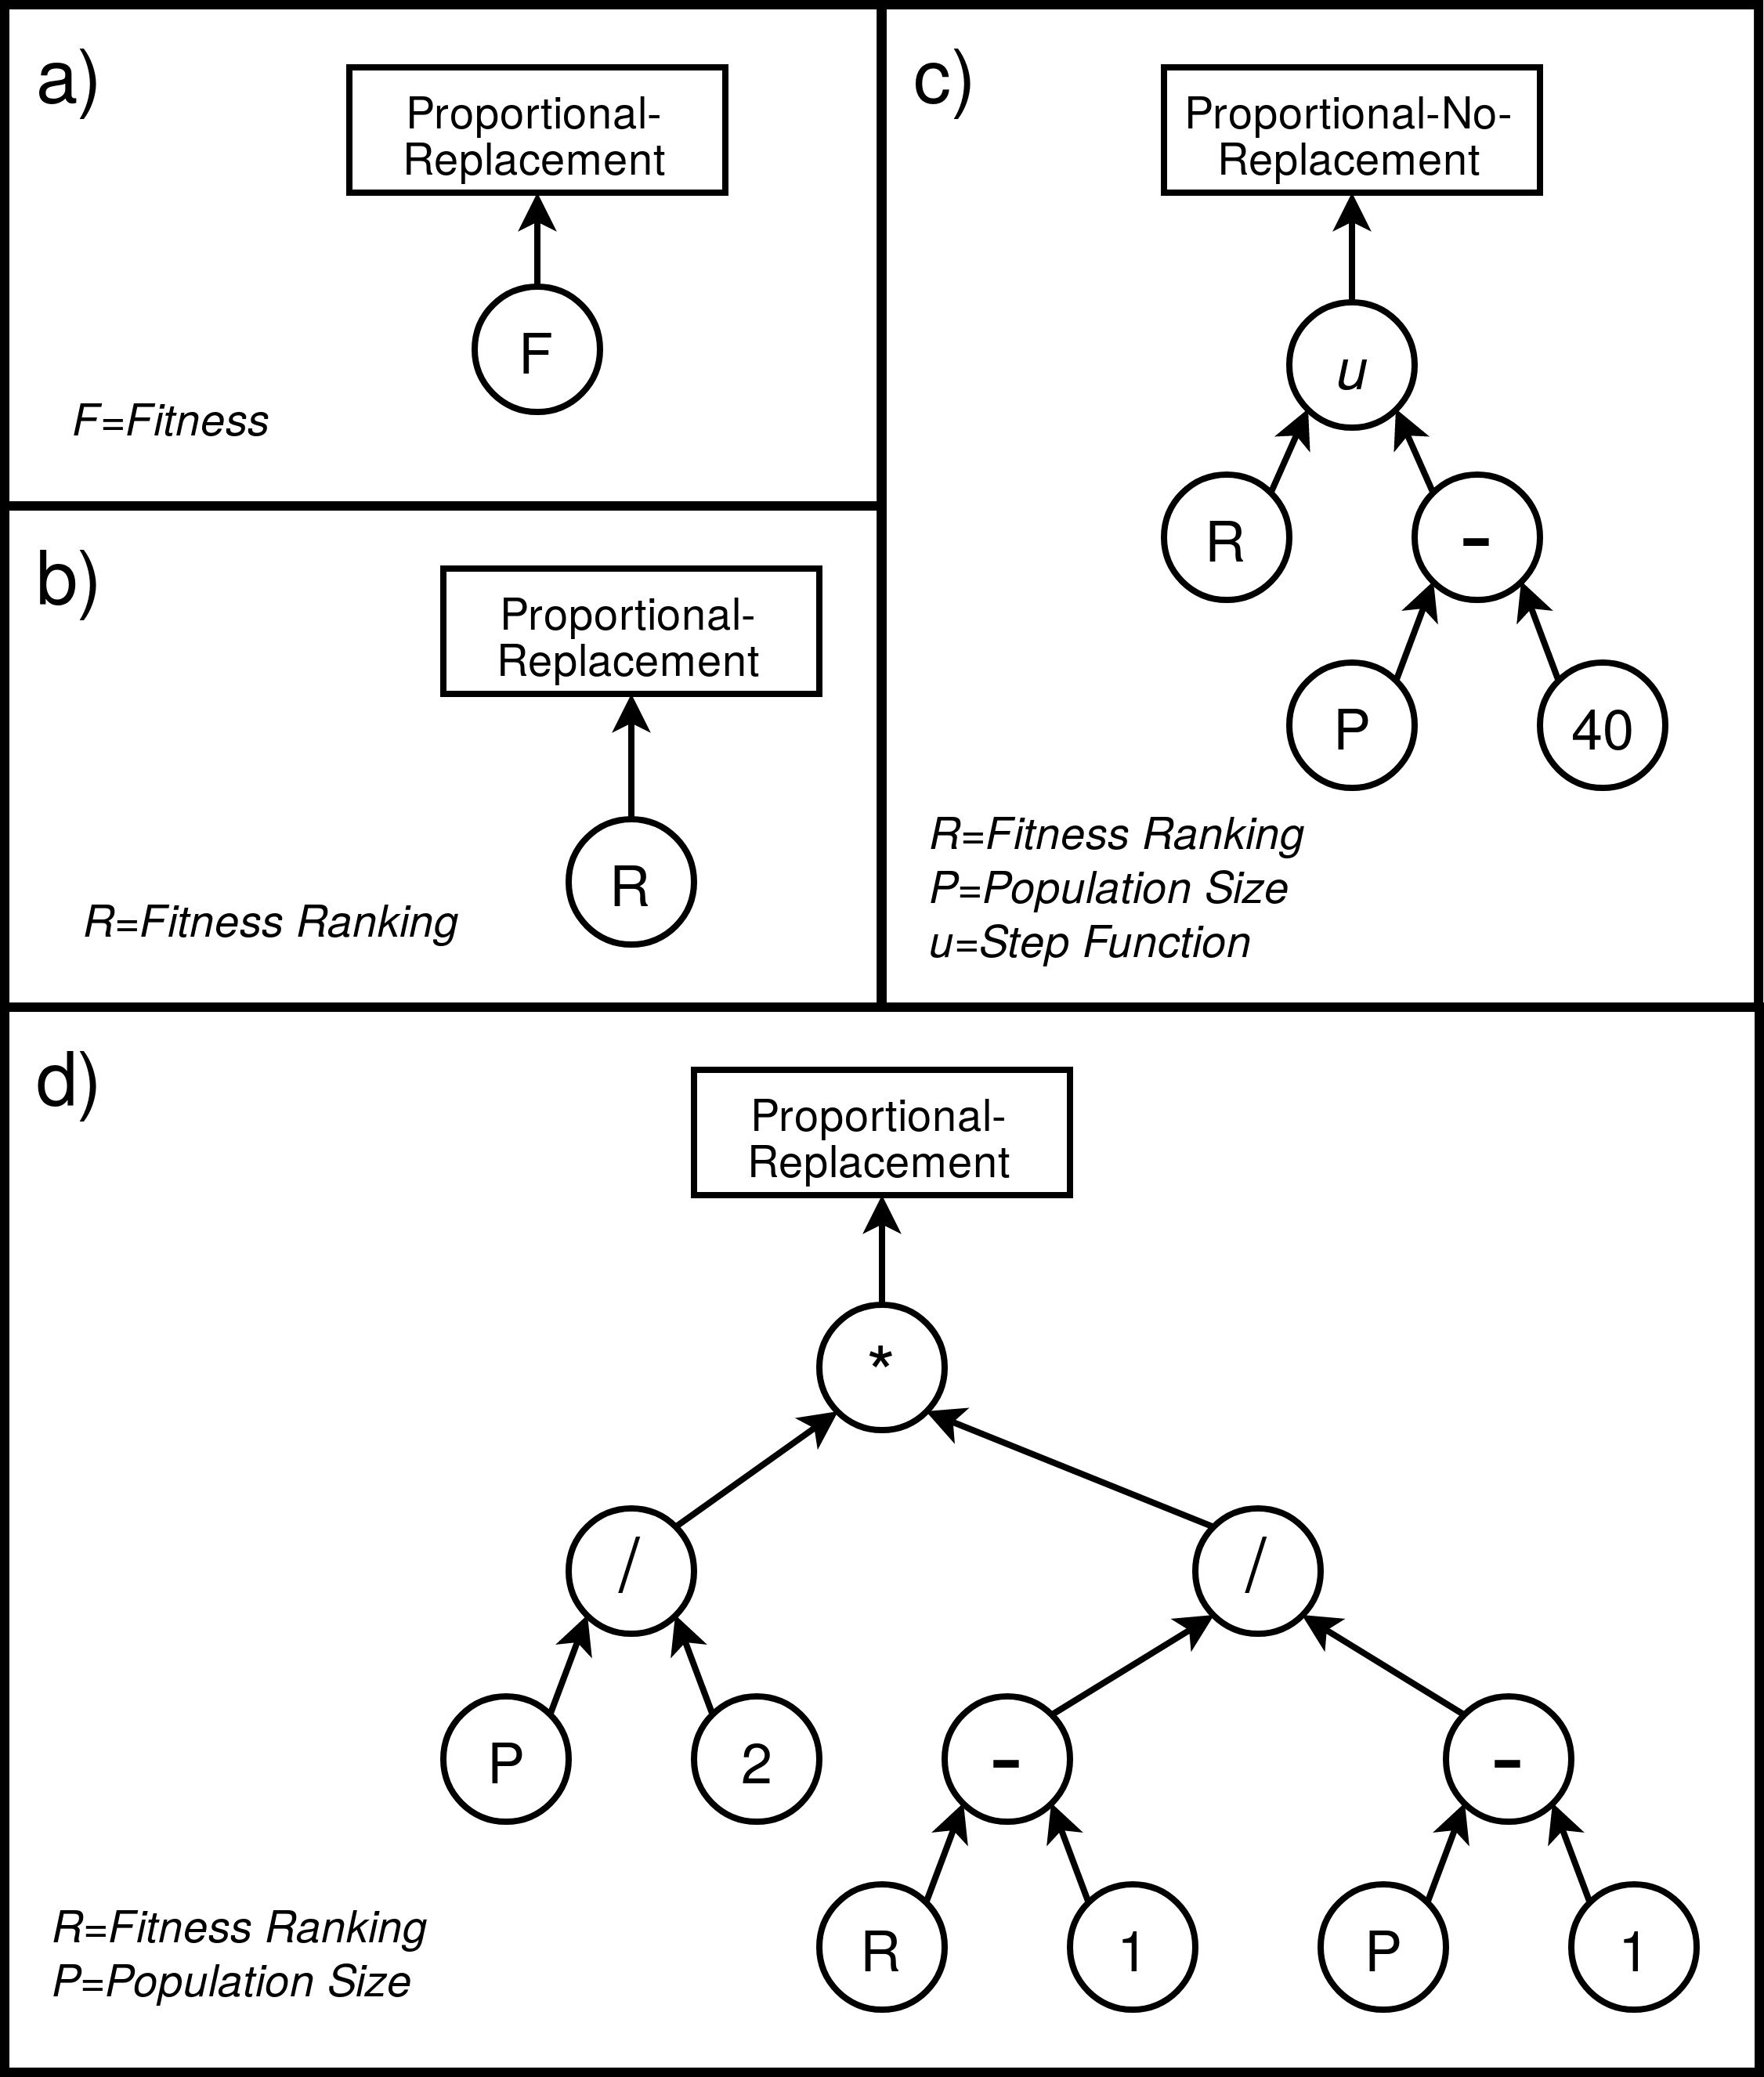
\includegraphics[width=0.9\textwidth]{old_eppsea_representation}
    \caption{The GP-Trees encoding the selection probabilities for typical selection functions, including a) Fitness proportional, b) Fitness Ranking, c) Truncation (T=40), and d) \textit{k}-tournament (\textit{k}=2).}
    \label{fig:old_eppsea_representation}
\end{figure}

\end{ThesisAppendix}

 % ... references - comma separated list of bib files ...

\begin{ThesisBibliography}{REFERENCES}
 %\bibliographystyle{unsrtnat}
 %\bibliographystyle{ieeetr}
 %\bibliographystyle{plainnat}
\bibliographystyle{mstogs}
\singlespacing
\bibliography{eppsea_bibliography}
\end{ThesisBibliography}

 % ... vita ...

\begin{Vita}
Samuel Richter was born and raised in St. Louis, Missouri. He enrolled at the Missouri University of Science and Technology in Fall 2012, working towards a Bachelor's Degree in Computer Engineering. In his senior year, he joined the Natural Computation Laboratory, where he was exposed to S\&T's state-of-the-art research in the field of evolutionary computing. After receiving his Bachelor's Degree in Spring 2016, he enrolled for a Master's Degree in Computer Science, which he earned in Fall 2018.
\end{Vita}

\end{document}

